%%% use 10pt options with the asme2ej format
%\documentclass[10pt]{asme2ej}
\documentclass[]{interact}

\usepackage{graphicx,epsfig,color,textcomp,amssymb,amsmath,mathrsfs,cancel,bbm,ulem,physics}

\usepackage{natbib}% Citation support using natbib.sty
\bibpunct[, ]{(}{)}{;}{a}{}{,}% Citation support using natbib.sty
\renewcommand\bibfont{\fontsize{10}{12}\selectfont}% Bibliography support using natbib.sty

\newcommand{\blue}[1]{\textcolor{blue}{[#1]}}
\newcommand{\red}[1]{\textcolor{red}{[#1]}}
\newcommand{\green}[1]{\textcolor{green}{[#1]}}
%\newcommand{\citepnum}[1]{\citep{[#1]}}
%% The class has several options
%  onecolumn/twocolumn - format for one or two columns per page
%  10pt/11pt/12pt - use 10, 11, or 12 point font
%  oneside/twoside - format for oneside/twosided printing
%  final/draft - format for final/draft copy
%  cleanfoot - take out copyright info in footer leave page number
%  cleanhead - take out the conference banner on the title page
%  titlepage/notitlepage - put in titlepage or leave out titlepage
%  
%% The default is oneside, onecolumn, 10pt, final


\title{Image-based multi-scale Mechanical Analysis of Strain Amplification as a Damage Mechanism of Neurons in a Collagen Gel}

\author{
\name{Victor W. L. Chan\textsuperscript{a},  William R. Tobin\textsuperscript{a}, Sijia Zhang\textsuperscript{b}, Beth A. Winkelstein\textsuperscript{b}, Victor H. Barocas\textsuperscript{c}, Mark S. Shephard\textsuperscript{a}, Catalin R. Picu\textsuperscript{a,d}\thanks{Corresponding Author: Catalin R. Picu, Tel: +518 276-2195, E-mail: picuc@rpi.edu}}
\affil{\textsuperscript{a}Scientific Computational Research Center, Rensselaer Polytechnic Institute, Low Center for Industrial Innocation, Troy, NY 12180; \\ \textsuperscript{b}Department of Bioengineering, University of Pennsylvania, Philadelphia, PA 19104; \\ \textsuperscript{c}Department of Biomedical Engineering, University of Minnesota, Minneapolis, MN 55455; \\ \textsuperscript{d}Department of Mechanical, Aerospace and Nuclear Engineering, Rensselaer Polytechnic Institute, Troy, NY 12180 } }

%%%% first author
%\author{Victor W. L. Chan
%    \affiliation{
%	Scientific Computation Research Center,\\
%	Rensselaer Polytechnic Institute,\\
%	Low Center for Industrial Innovation, CII-4011,\\
%	110 8th Street,\\
%	Troy, NY 12180
%    }	
%}
%
%%%% second author
%%%% remove the following entry for single author papers
%%%% add more entries for additional authors
%\author{William R. Tobin 
%    \affiliation{ Scientific Computation Research Center,\\
%	Rensselaer Polytechnic Institute,\\
%	Low Center for Industrial Innovation, CII-4011,\\
%	110 8th Street,\\
%	Troy, NY 12180
%    }
%}
%
%%%% third author
%%%% remove the following entry for single author papers
%%%% add more entries for additional authors
%\author{Sijia Zhang
%    \affiliation{ Department of Bioengineering,\\
%        University of Pennsylvania,\\
%	240 Skirkanich Hall,\\
%        210 South 33rd Street,\\
%         Philadelphia, PA 19104
%    }
%}
%
%\author{Beth A. Winkelstein
%    \affiliation{ Department of Bioengineering,\\
%        University of Pennsylvania,\\
%	240 Skirkanich Hall,\\
%        210 South 33rd Street,\\
%         Philadelphia, PA 19104
%    }
%}
%
%\author{Victor H. Barocas
%    \affiliation{ Department of Biomedical Engineering,\\
%        University of Minnesota,\\
%	7-105 Nils Hasselmo Hall,\\
%        312 Church Street SE,\\
%        Minneapolis, MN 55455
%    }
%}
%
%\author{Mark S. Shephard
%    \affiliation{ Scientific Computation Research Center,\\
%	Rensselaer Polytechnic Institute,\\
%	Low Center for Industrial Innovation, \\
%	CII-4011, 110 8th Street,\\
%	Troy, NY 12180
%    }
%}
%
%\author{Catalin R. Picu
%       \thanks{Address all correspondence for other issues to this author.} 
%        \affiliation{Scientific Computation Research Center,\\
%	Rensselaer Polytechnic Institute,\\
%	Low Center for Industrial Innovation, \\
%	CII-4011, 110 8th Street,\\
%	Troy, NY 12180; \\
%	Department of Mechanical, Aerospace and Nuclear Engineering, \\
%	Rensselaer Polytechnic Institute, \\
%	Jonsson Engineering Center,\\
%	Rm.\ 2049, 110 8th Street, \\
%	Troy, NY 12180 \\
%	email: picuc@rpi.edu
%    }
%}



\begin{document}

\maketitle    

%%%%%%%%%%%%%%%%%%%%%%%%%%%%%%%%%%%%%%%%%%%%%%%%%%%%%%%%%%%%%%%%%%%%%%
\begin{abstract}
{\it 
Needs to be filled in.
}
\end{abstract}

%%%%%%%%%%%%%%%%%%%%%%%%%%%%%%%%%%%%%%%%%%%%%%%%%%%%%%%%%%%%%%%%%%%%%%
\section{Introduction}

In early studies of tissue mechanics \citep{Fung1993}, the focus was on developing constitutive equations that described the mechanical behavior of a tissue as a continuous, homogeneous entity. Even the continuous tissue mechanics problem is extremely difficult, with issues such as viscoelasticity [\red{reference}], nonlinearity [\red{reference}], multiphasicity [\red{reference}], anisotropy [\red{reference}], active stress generation [\red{reference}], damage [\red{reference}], and growth and remodeling [\red{reference}] all coming into play under various circumstances. Much of the work in the previous century of biomechanics has attempted to capture these different complexities, and this is the level at which to attack many problems given the macroscopic nature of humans and the apparent continuity of the tissue when viewed on the macroscopic scale.

More recently, however, it has been recognized that the essential unit that responds to a macroscopic load is in fact microscopic, such as a smooth-muscle in a growing aneurysm [\red{reference}], a somatosensory nerve ending [\red{reference}], a chondrocyte remodeling the surrounding tissue [\red{reference}], a cell remodeling its scaffold in an engineered blood vessel [\red{reference}], or - most relevant to the current work - a neurite being injured by excessive stretch [\red{reference}]. In each of these cases, a macroscopic/tissue-scale loading condition is transferred to the microscopic/cell-scale stress, which in turn drives the response. If we hope to understand the microscopic response to a macroscopic load, a scale-bridging strategy is clearly needed.

The constrained-mixture models \citep{Humphrey:2002ga} have been extremely effective in predicting growth and remodeling at the continuum scale, but they do not account for the local cell stress that arises, treating the cells instead as a continuous component of a mixture. As such, constrained-mixture models are not designed to address the effect of local strain field variations due to the presence of a cell, as observed experimentally in fibroblast-populated collagen gels \red{[Voytik-Harbin]}. 

Inspired by classic work in the theory of composite materials \citep{Hashin:1962tm}, numerous studies have now been made where models are constructed of a cell surrounded by acellular material. In most cases [\red{references}], the approach employed is to place a cell of idealized shape (sphere or ellipsoid) in the center of the cube. A notable extension is the multi-cell simulations of Marquez, Genin, and Elson \citep{Marquez:2006gv}, in which cylindrical or ellipsoidal cells were progressively added to the system, and a jump in effect was observed when the cells percolated the domain.  Another contribution \citep{Lai:2013fp} was the replacement of the closed-form constitutive equation with a multi-scale model that allows better representation of the extracellular matrix structure.

In spite of these recent advances, there is still considerably more work to be done in pursuing a realistic representation of the cell's or tumor's mechanical environment under a given tissue load. Perhaps the most salient missing feature of current models is the fact that the microscopic entity is rarely spherical in shape.  For example, fibroblasts spread and polarize within a collagen matrix [\red{reference}], and a malignant tumor can have an extremely complex geometry [Cristini?]. There is a compelling need for methods that can account for the detailed microscale geometry when downscaling mechanical information.

Major barriers to a realistic representation of complex cell geometry include the generation of a model geometry from experimentally measured images and the subsequent mesh generation on that model geometry. Furthermore, the number of degrees of freedom required to properly represent the morphology of a complex cell geometry is large, and when coupled with a multi-scale framework, the computational demand can become prohibitive. 

In this work, we addressed some of these challenges by developing a multi-scale model of a group of neurons that are embedded within a collageneous matrix. Our objective in this work was to develop a general modeling strategy in which (1) confocal microscopy or another three-dimensional imaging modality is used to generate a realistic representation of a complex cell geometry, (2) that geometric model, along with the surrounding extracellular matrix, is converted to a finite-element mesh, (3) a multi-scale model is implemented on that mesh using a network microstructural model at each Gauss point \citep{Chandran:2007hy,Stylianopoulos:2007dp}, and (4) the solution of the mechanics problem is used to determine the distribution of strains within the cell. 

Although the approach described herein is general, it is focused on the specific experimental system of dorsal root ganglion (DRG) neurons embedded in a collagen gel. This model system, which has been used extensively by the Winkelstein group [\red{reference}] and others [\red{reference}], allows detailed study of the cellular mechanisms of neuronal injury in a more controllable environment than can be achieved in vivo. As such, it has the potential to provide insight into the mechanism of neuronal injury under mechanical load, with biochemical markers of neuronal injury being quantified in response to different macroscopic strains and/or strain rates \citep{Zhang:2016ga}. 

To test the method, we applied it to images taken of an embedded neuron in gel system \citep{Zhang:2016ga}. To summarize this system, neurons were embedded in collagen gels to mimic the innervation of ligamentous tissue, such as those found in the spinal facet capsular ligament \citep{McLain1998RF,Kallakuri:2012ib} and the knee joint capsule \citep{Schultz1984RA,Khalsa:CKPnLlfY}. This in vitro system has been utilized to study the effects of macroscopic and microscopic scale tissue mechanics on neuronal responses in the context of ligament pain. Previous studies using this and similar neuron-collagen culture models suggest that neuronal activation and pain signaling can be modulated by the macroscopic strain and collagen organization of the surrounding extracellular matrix \citep{Zhang:2016ga, Zhang2017S}. However, this in vitro system does not enable detailed evaluation of neuronal mechanics, which is important for understanding the local mechanisms of neuronal mechanosensing and/or injury due to tissue loading. Therefore, an image-based multi-scale model that complements that neuron-collagen in vitro system is needed to investigate the relationships between macroscopic tissue deformations and mechanical changes in neurons. 

The complex geometry of the neurons are incorporated into our model by employing tools developed by Simmetrix Inc. \citep{simmetrix} that are capable of generating geometric models from experimental images \citep{Klaas_conference, Klaas:2013ug} and to mesh the resulting geometric model \citep{Shephard:2000vc}. Additionally, the large computational demands of a multi-scale model on the resulting mesh are accommodated by the adaptive multi-scale simulation infrastructure (AMSI) library \citep{Delalondre:2010kt,Tobin:2017ip}, which was designed to simultaneously handle massively parallel simulations on multiple scales.

%%%%%%%%%%%%%%%%%%%%%%%%%%%%%%%%%%%%%%%%%%%%%%%%%%%%%%%%%%%%%%%%%%%%%%
\section{Representation of Complex Cell Geometry}

A realistic representation of complex cell geometry was generated from three-dimensional (3D) voxelated data that originated from a stack of image slices. Noise in the voxelated data that results from the limited level of contrast in the imaging technique are removed using a combination of erosion/dilation, manual reassignment, small object removal, and smoothing operations which were applied using the \textit{ImageToModel} tool \citep{Klaas:2013ug, Klaas_conference, simmetrix}. Once processed, the voxelated data is converted into a discrete geometry via an initial triangulation that is based on voxel level operations where mesh coarsening is not performed until after the surface triangulation has been smoothed \citep{Klaas:2013ug}. Quantization artifacts on the surface of the geometry due to the voxel nature of the data are removed using a smoothing algorithm that consists of three steps \citep{Klaas:2013ug}: (i) calculate the surface normal of the desired surface geometry at each mesh face based on the normals of neighboring mesh faces; (ii) smooth surface normals on mesh to obtain the normals of desired surface geometry; (iii) iteratively adjust the mesh vertex positions to create a surface that matches the smoothed surface normals.

In this work, the input 3D voxelated data was constructed from confocal Z-stack images taken from an unloaded three-dimensional (3D) neuron-collagen culture system. Briefly, dorsal root ganglia were harvested from embryonic day 18 rats, dissociated and embedded in a collagen Type I gel (2mg/ml; Corning Inc; Corning, NY), using methods described in prior studies \citep{Cullen:2012gu, Zhang:2016ga, Zhang2017S}. The structure of neurons was visualized by fluorescence labeling of the cytoskeletal protein $\beta$III-tubulin (Abcam Cambridge, MA), as described previously \citep{Zhang:2016ga, Zhang2017S}. A Zeiss LSM 510 confocal microscope (Carl Zeiss Inc; Thornwood, NY) was used to image the neurons.  Z-stack images (2-micron thick) were taken at a resolution of 0.22$\mu$m/pixel with a 40X objective. Five consecutive images, each having a thickness of 2$\mu$m, were used to reconstruct the neuronal structure in 3D. All images were segmented using \textit{ImageJ} \citep{Schneider:2012dw} based on the positive labeling of $\beta$III-tubulin for model construction and speckle noise in the background was removed in Adobe Photoshop (Adobe Systems Incorporated; San Jose, CA).  The few raw confocal Z-stack images that were used in our model are shown in Fig.\ \ref{fig:Z-stack-images}. 
%
% Z-stack images from Neuron-in-gel-Analysis folder
\begin{figure}[ht]
\begin{center}
$
\begin{array}{ccc}
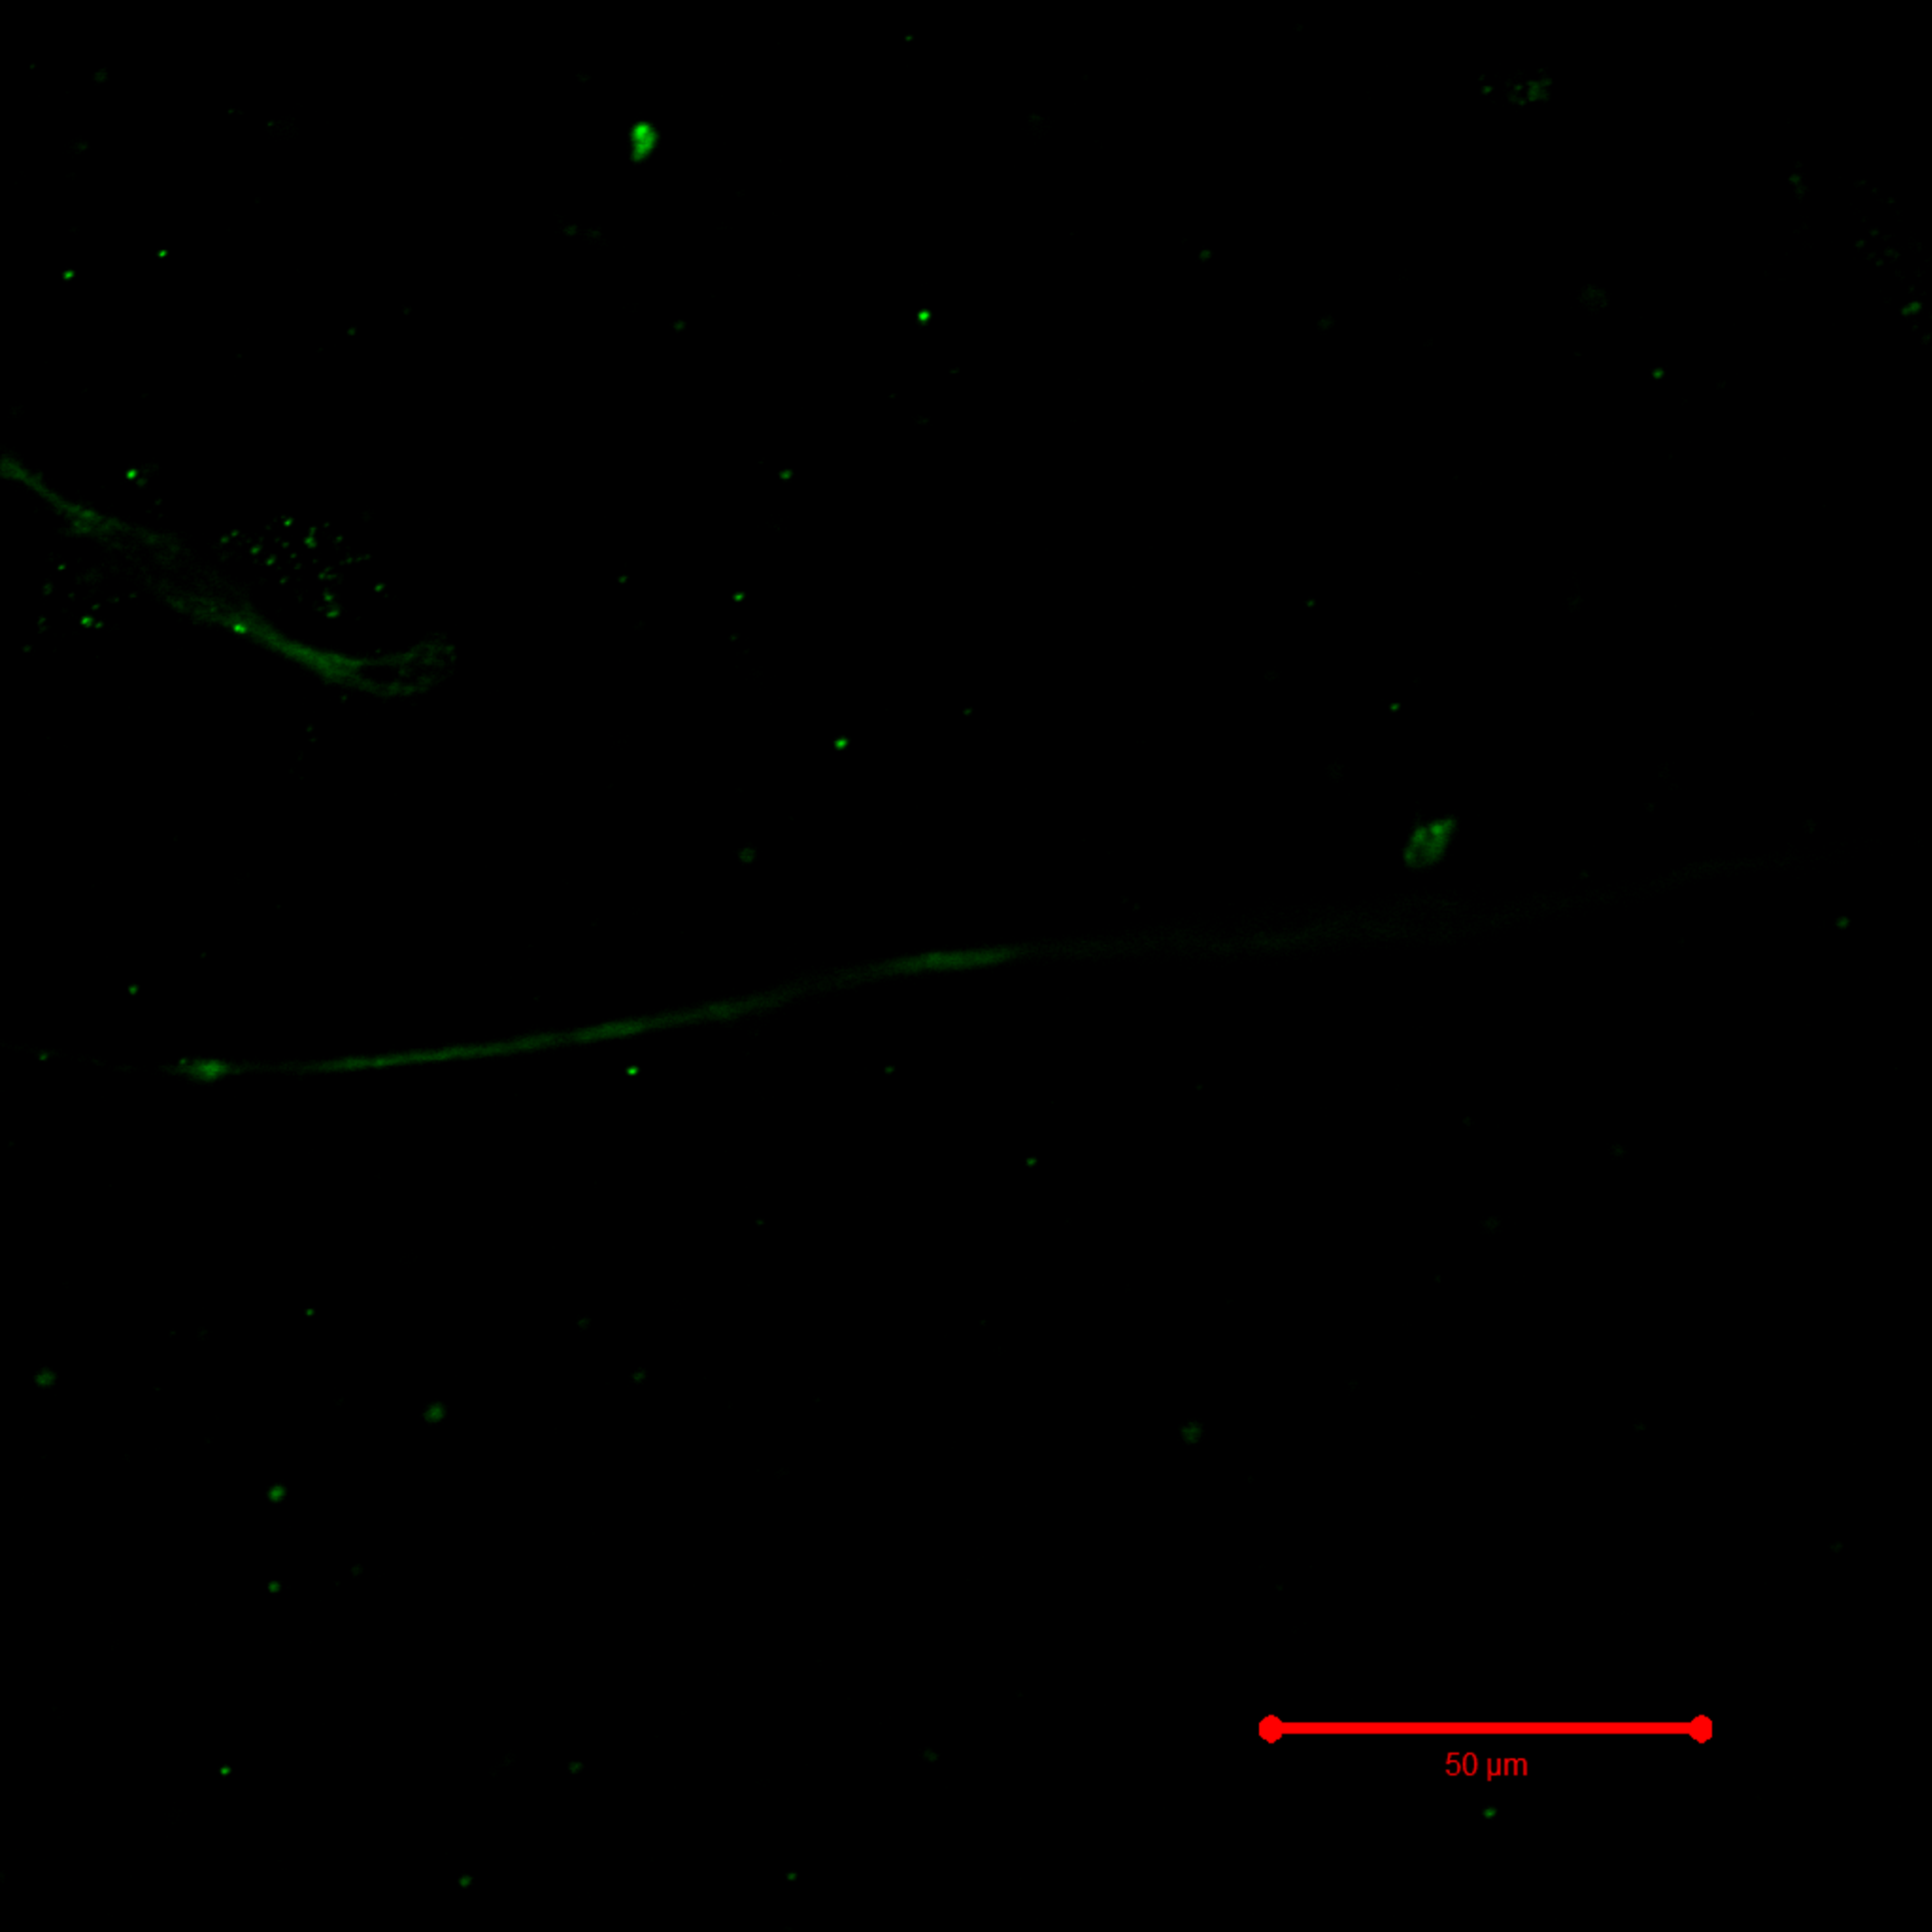
\includegraphics[height=4cm]{figure/neuron_image-scale-bar} & 
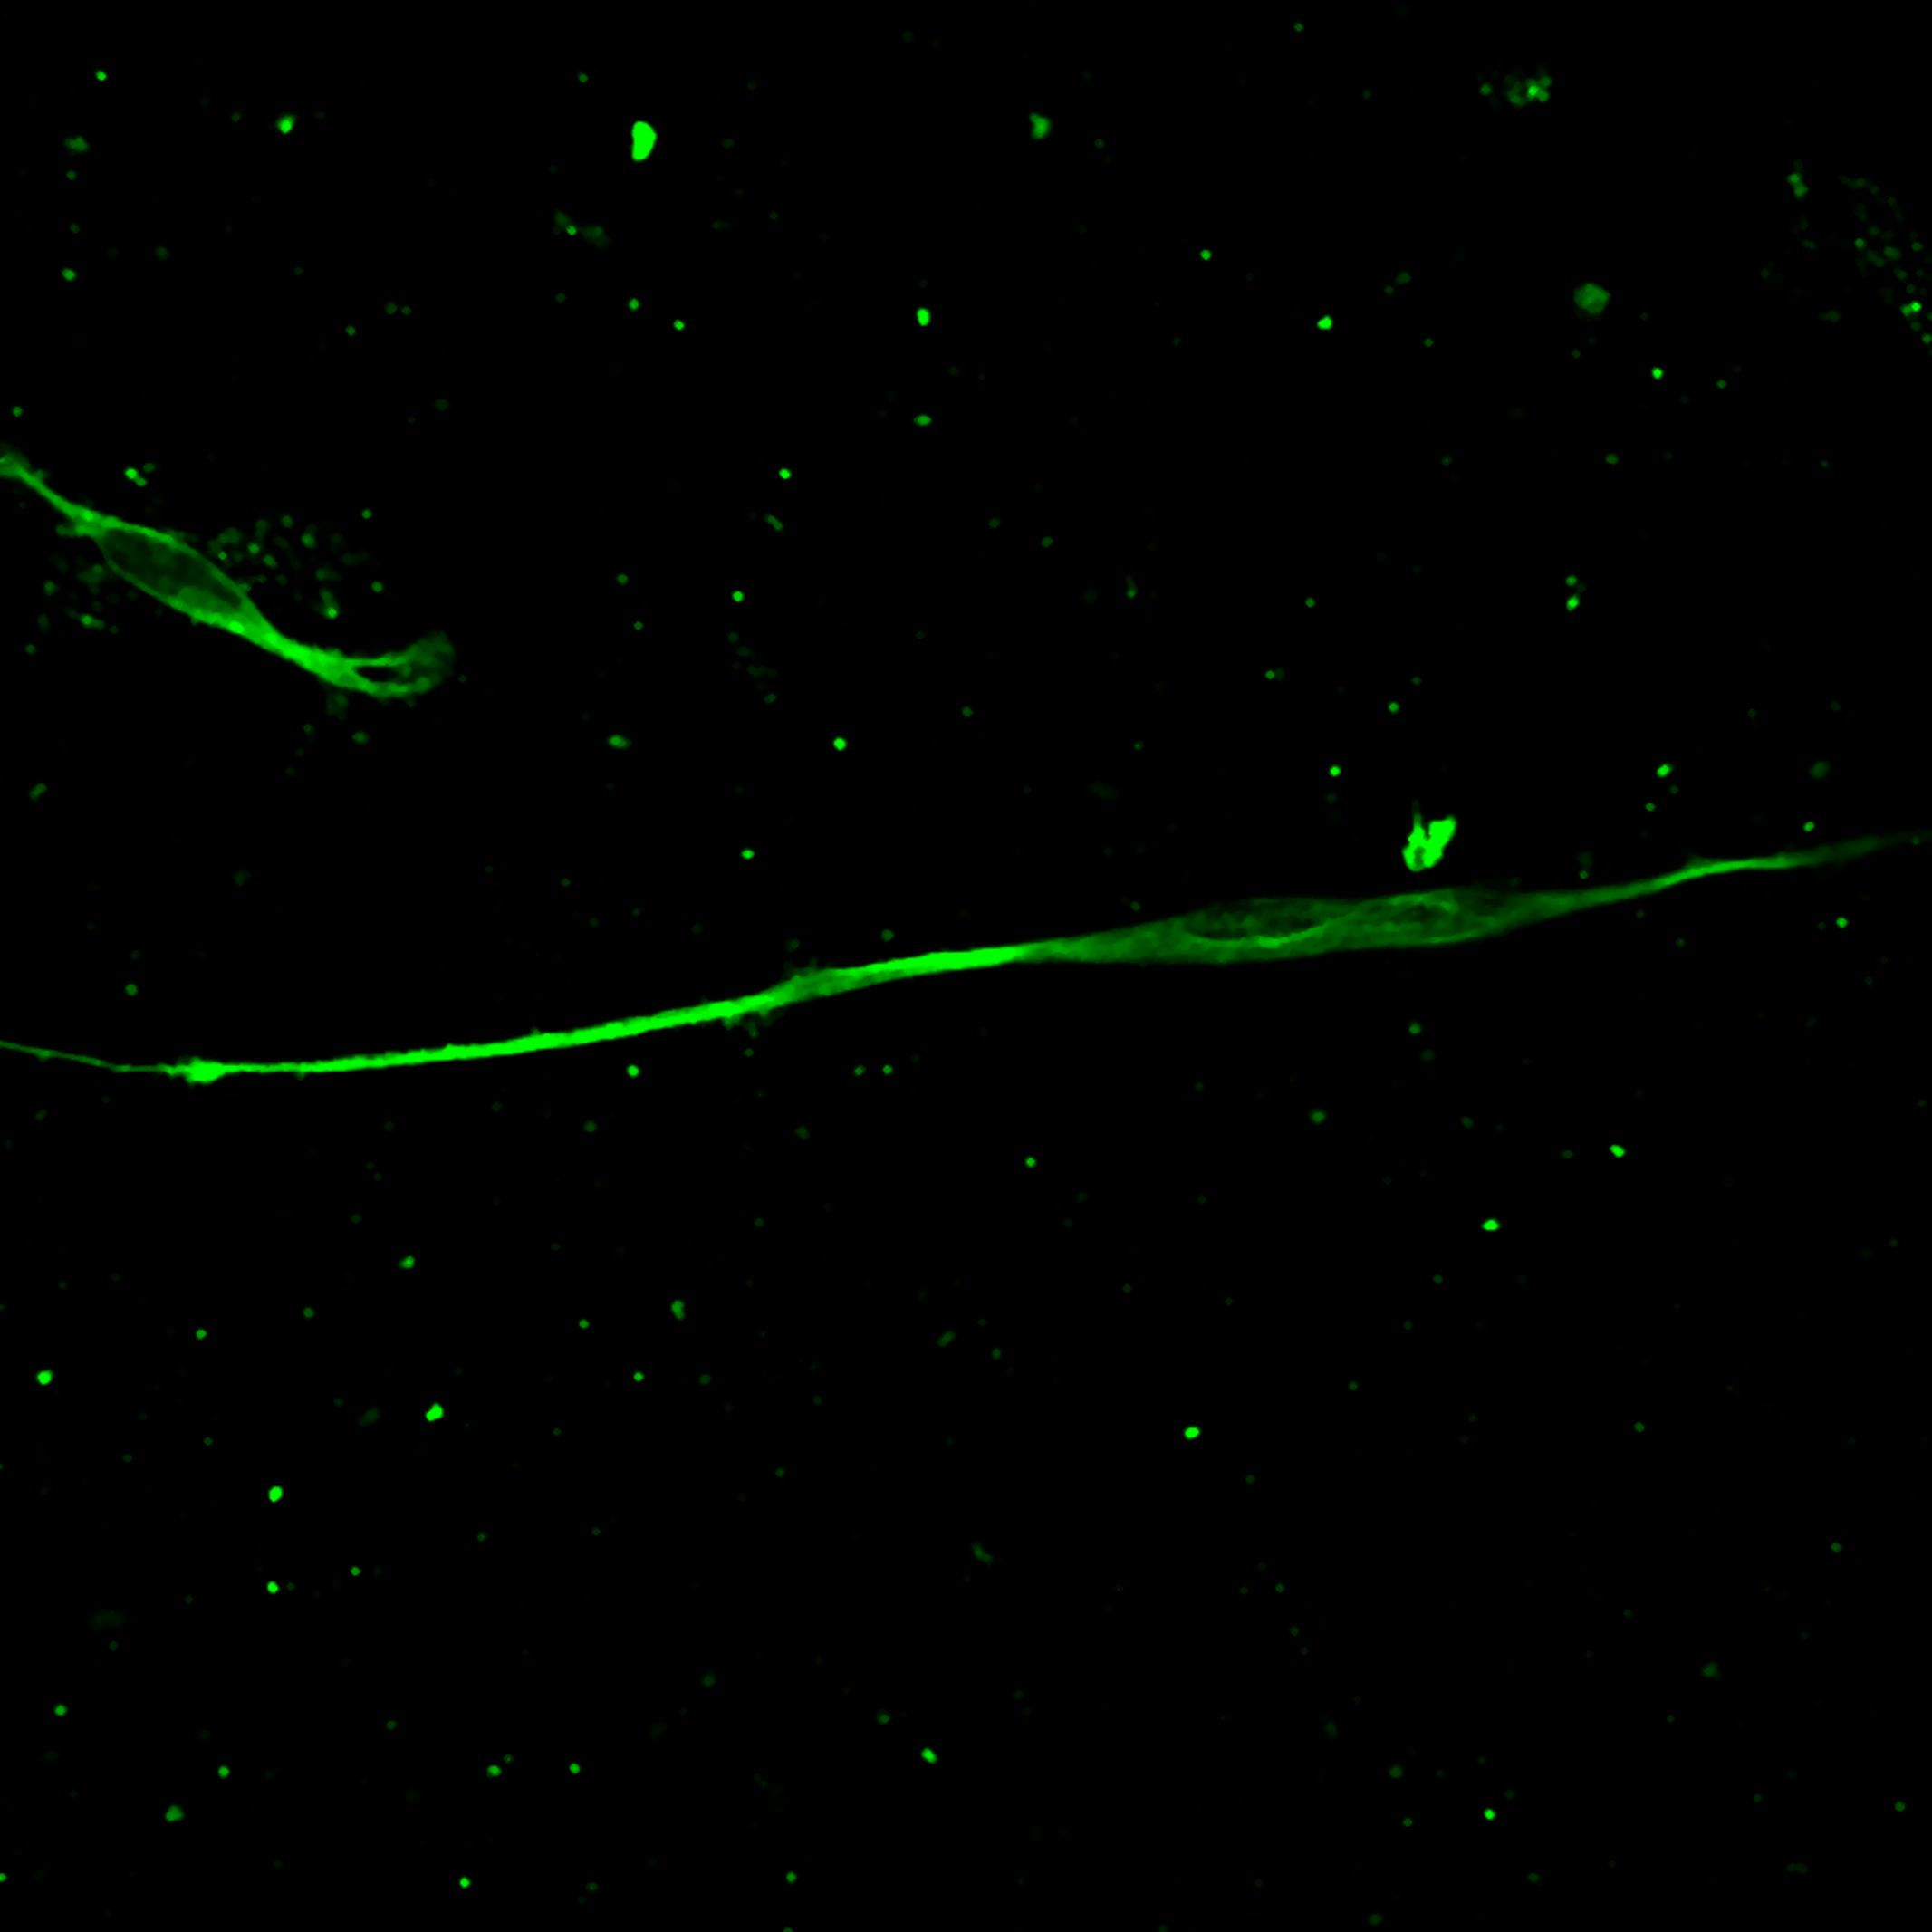
\includegraphics[height=4cm]{figure/neuron_image2} \\
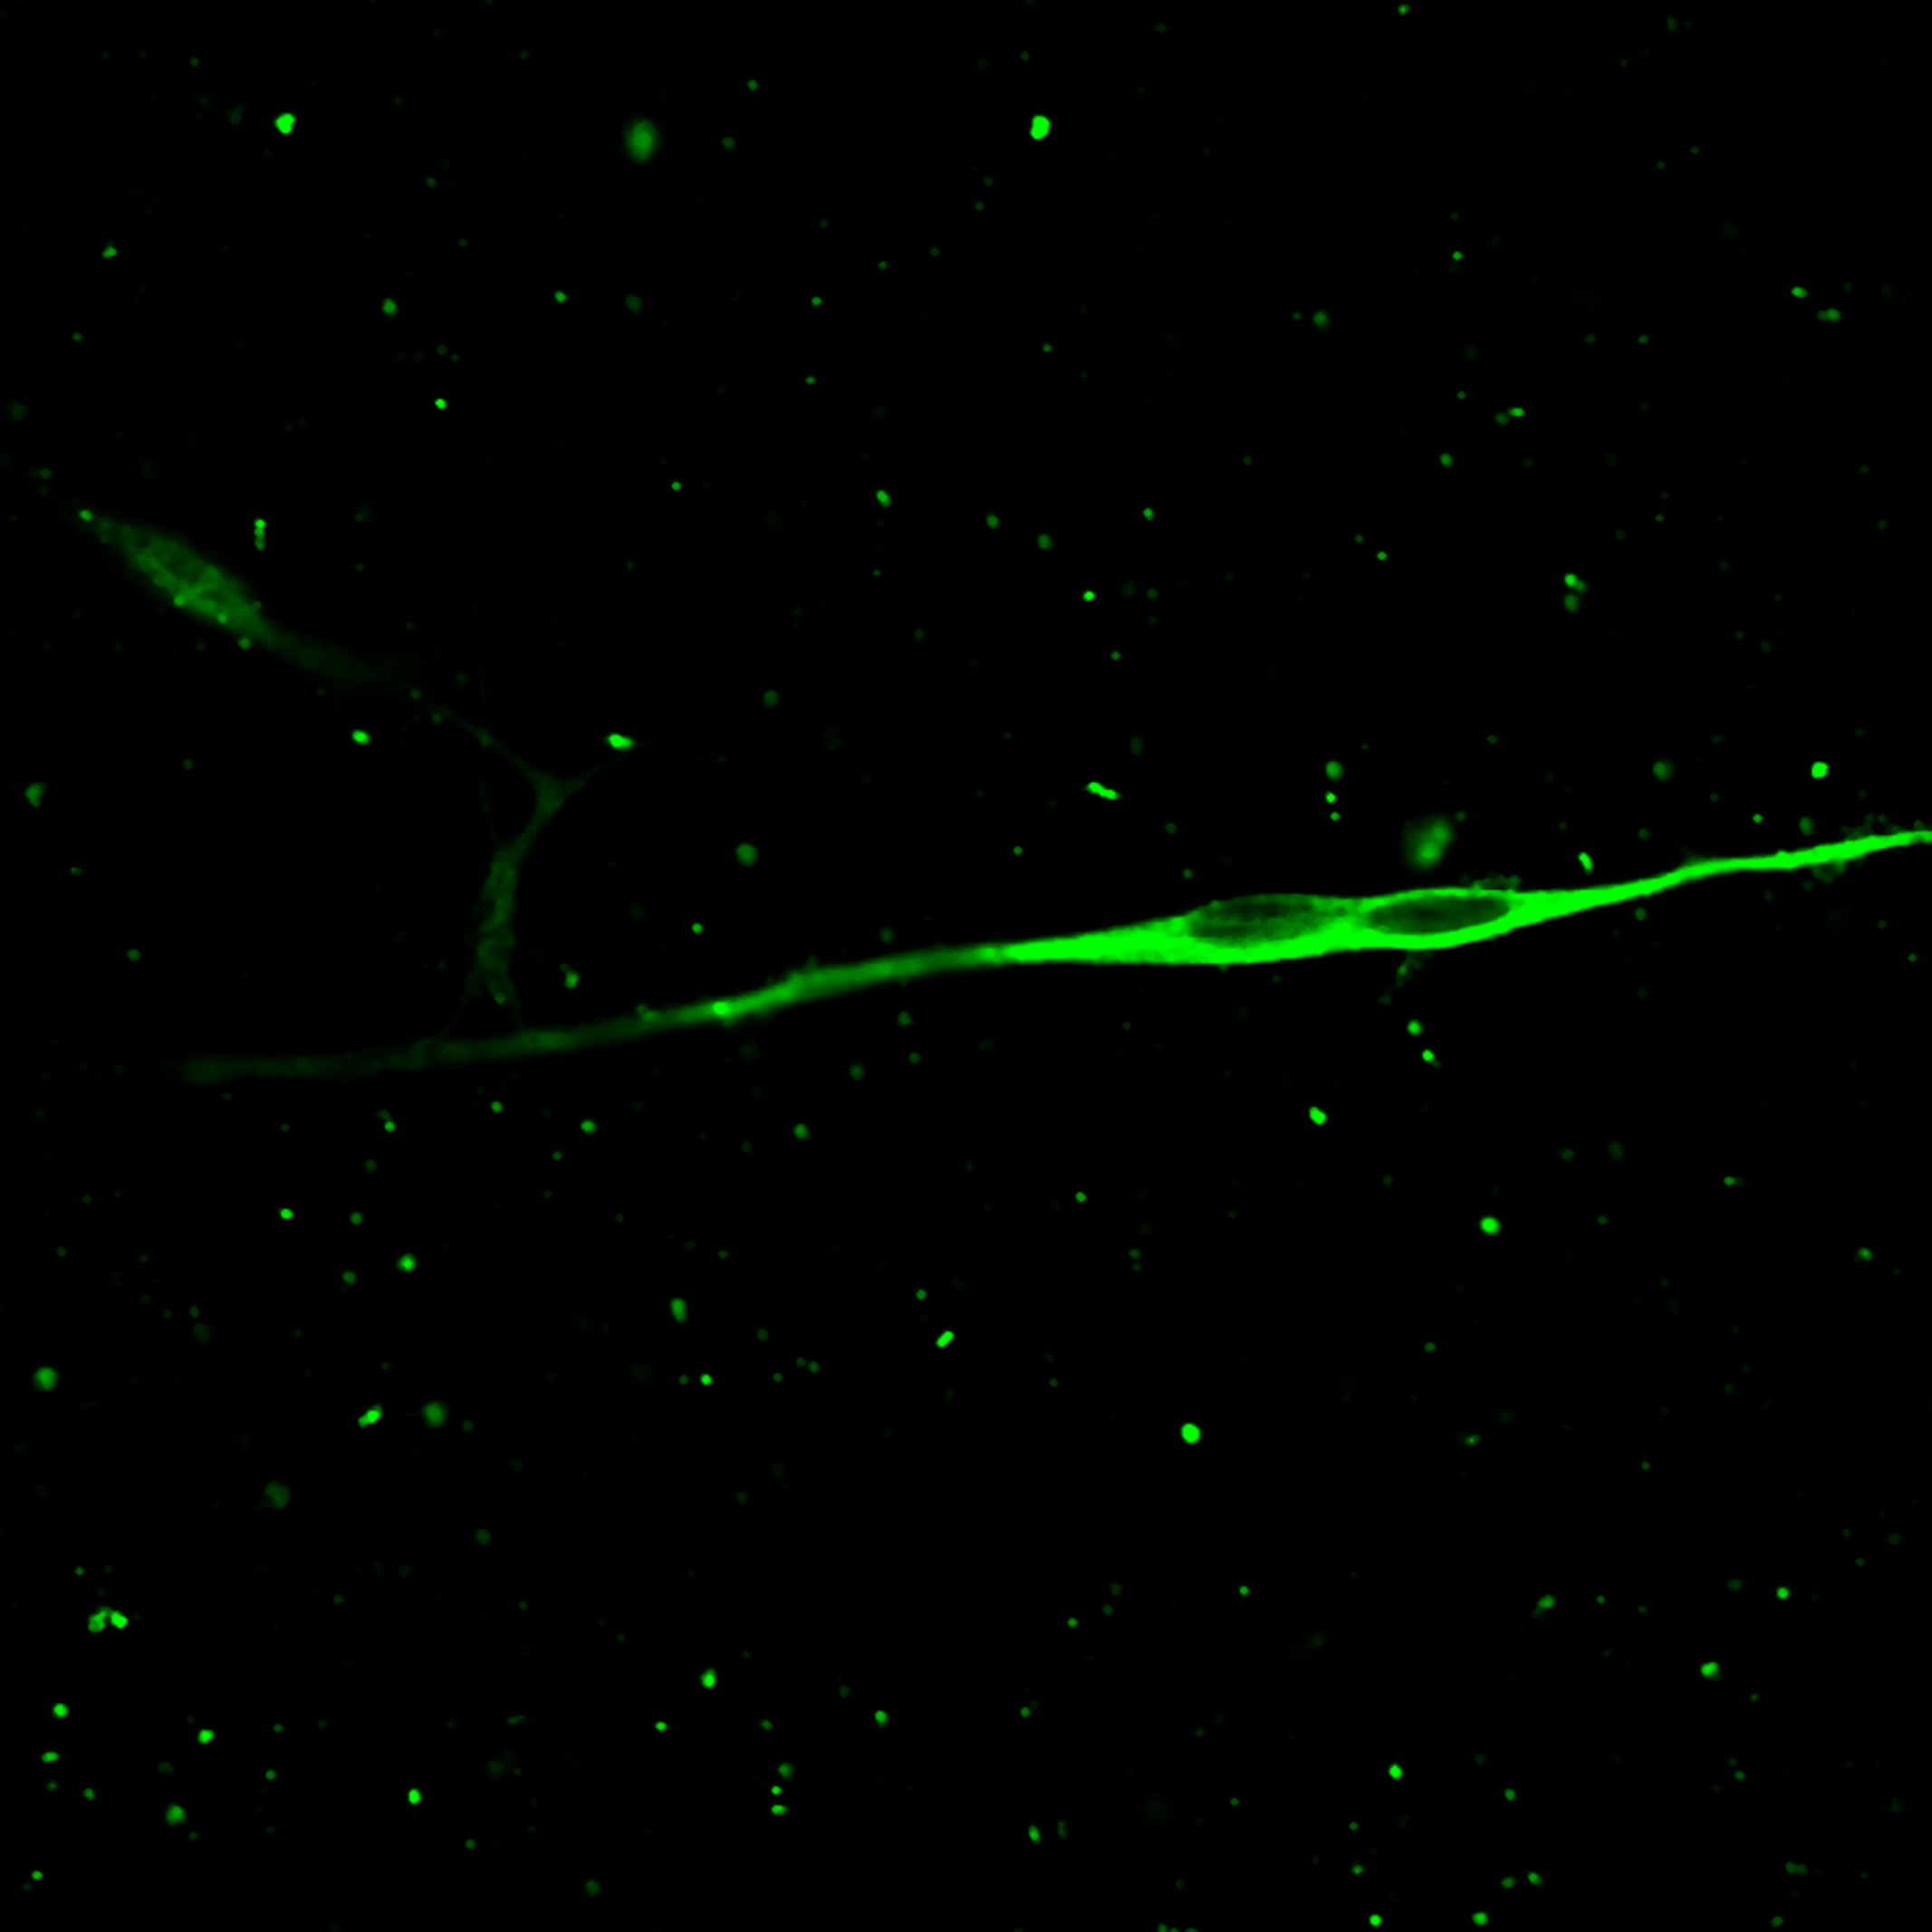
\includegraphics[height=4cm]{figure/neuron_image3} &
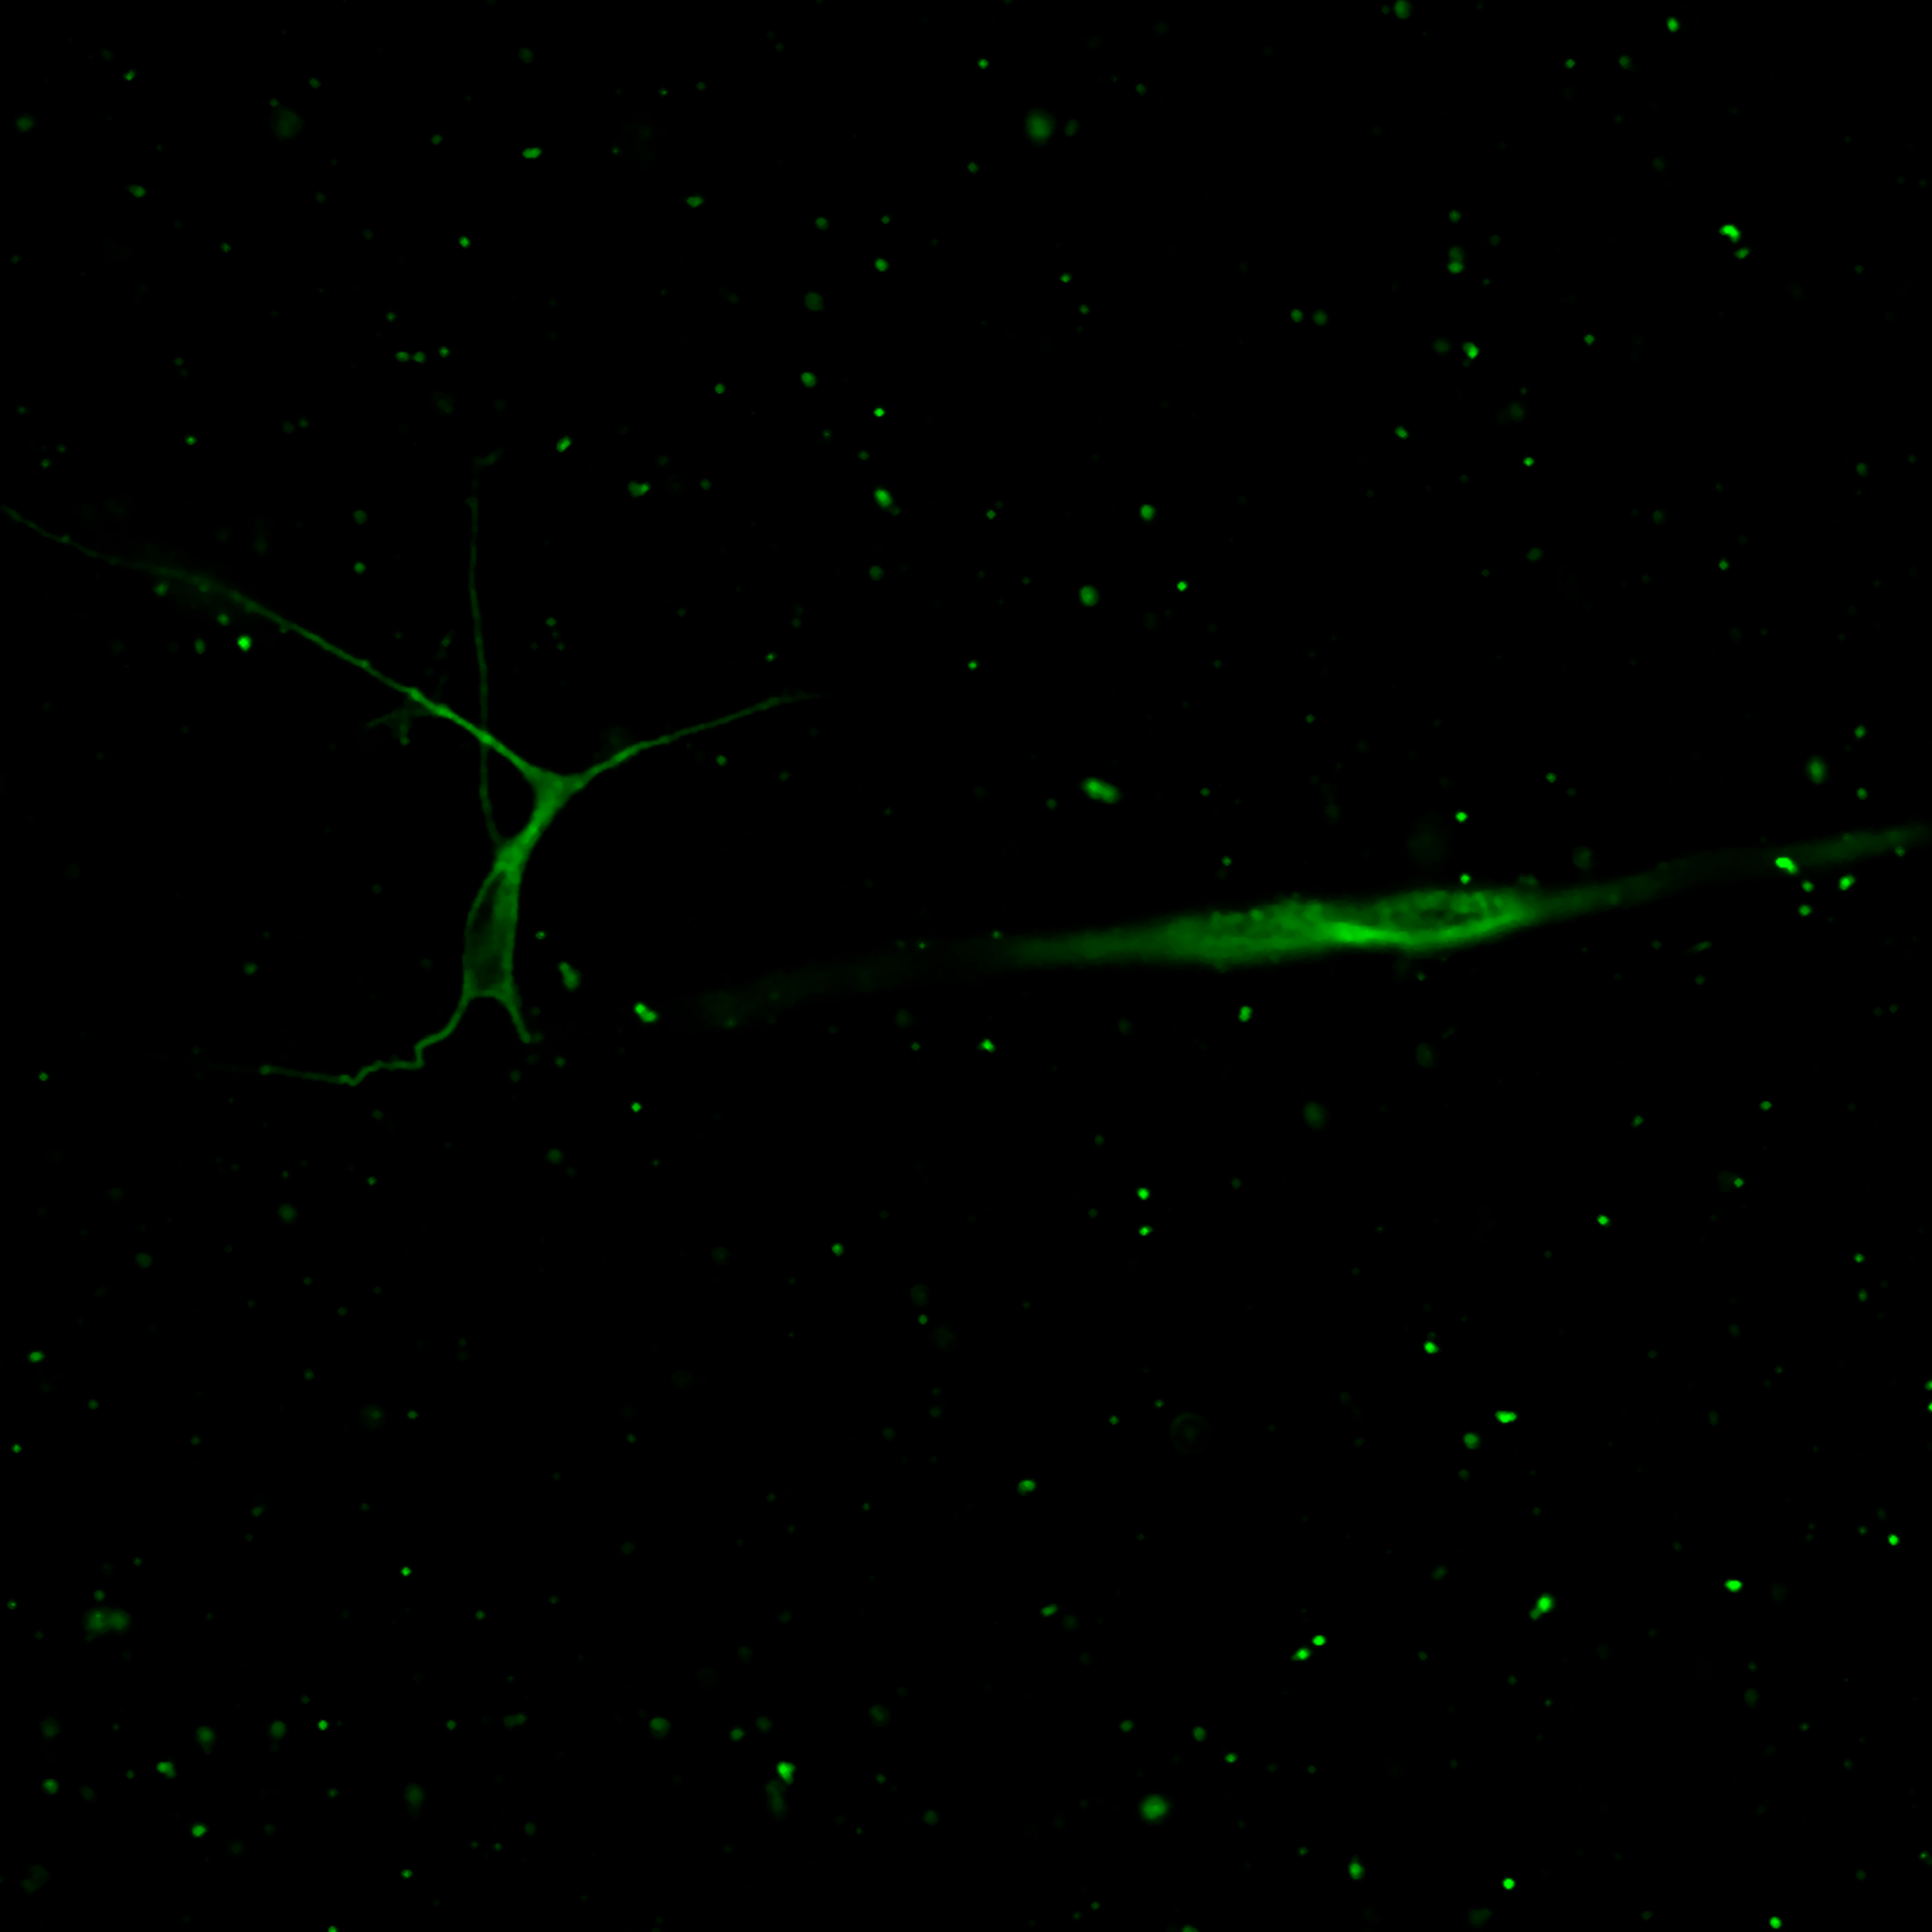
\includegraphics[height=4cm]{figure/neuron_image4} &
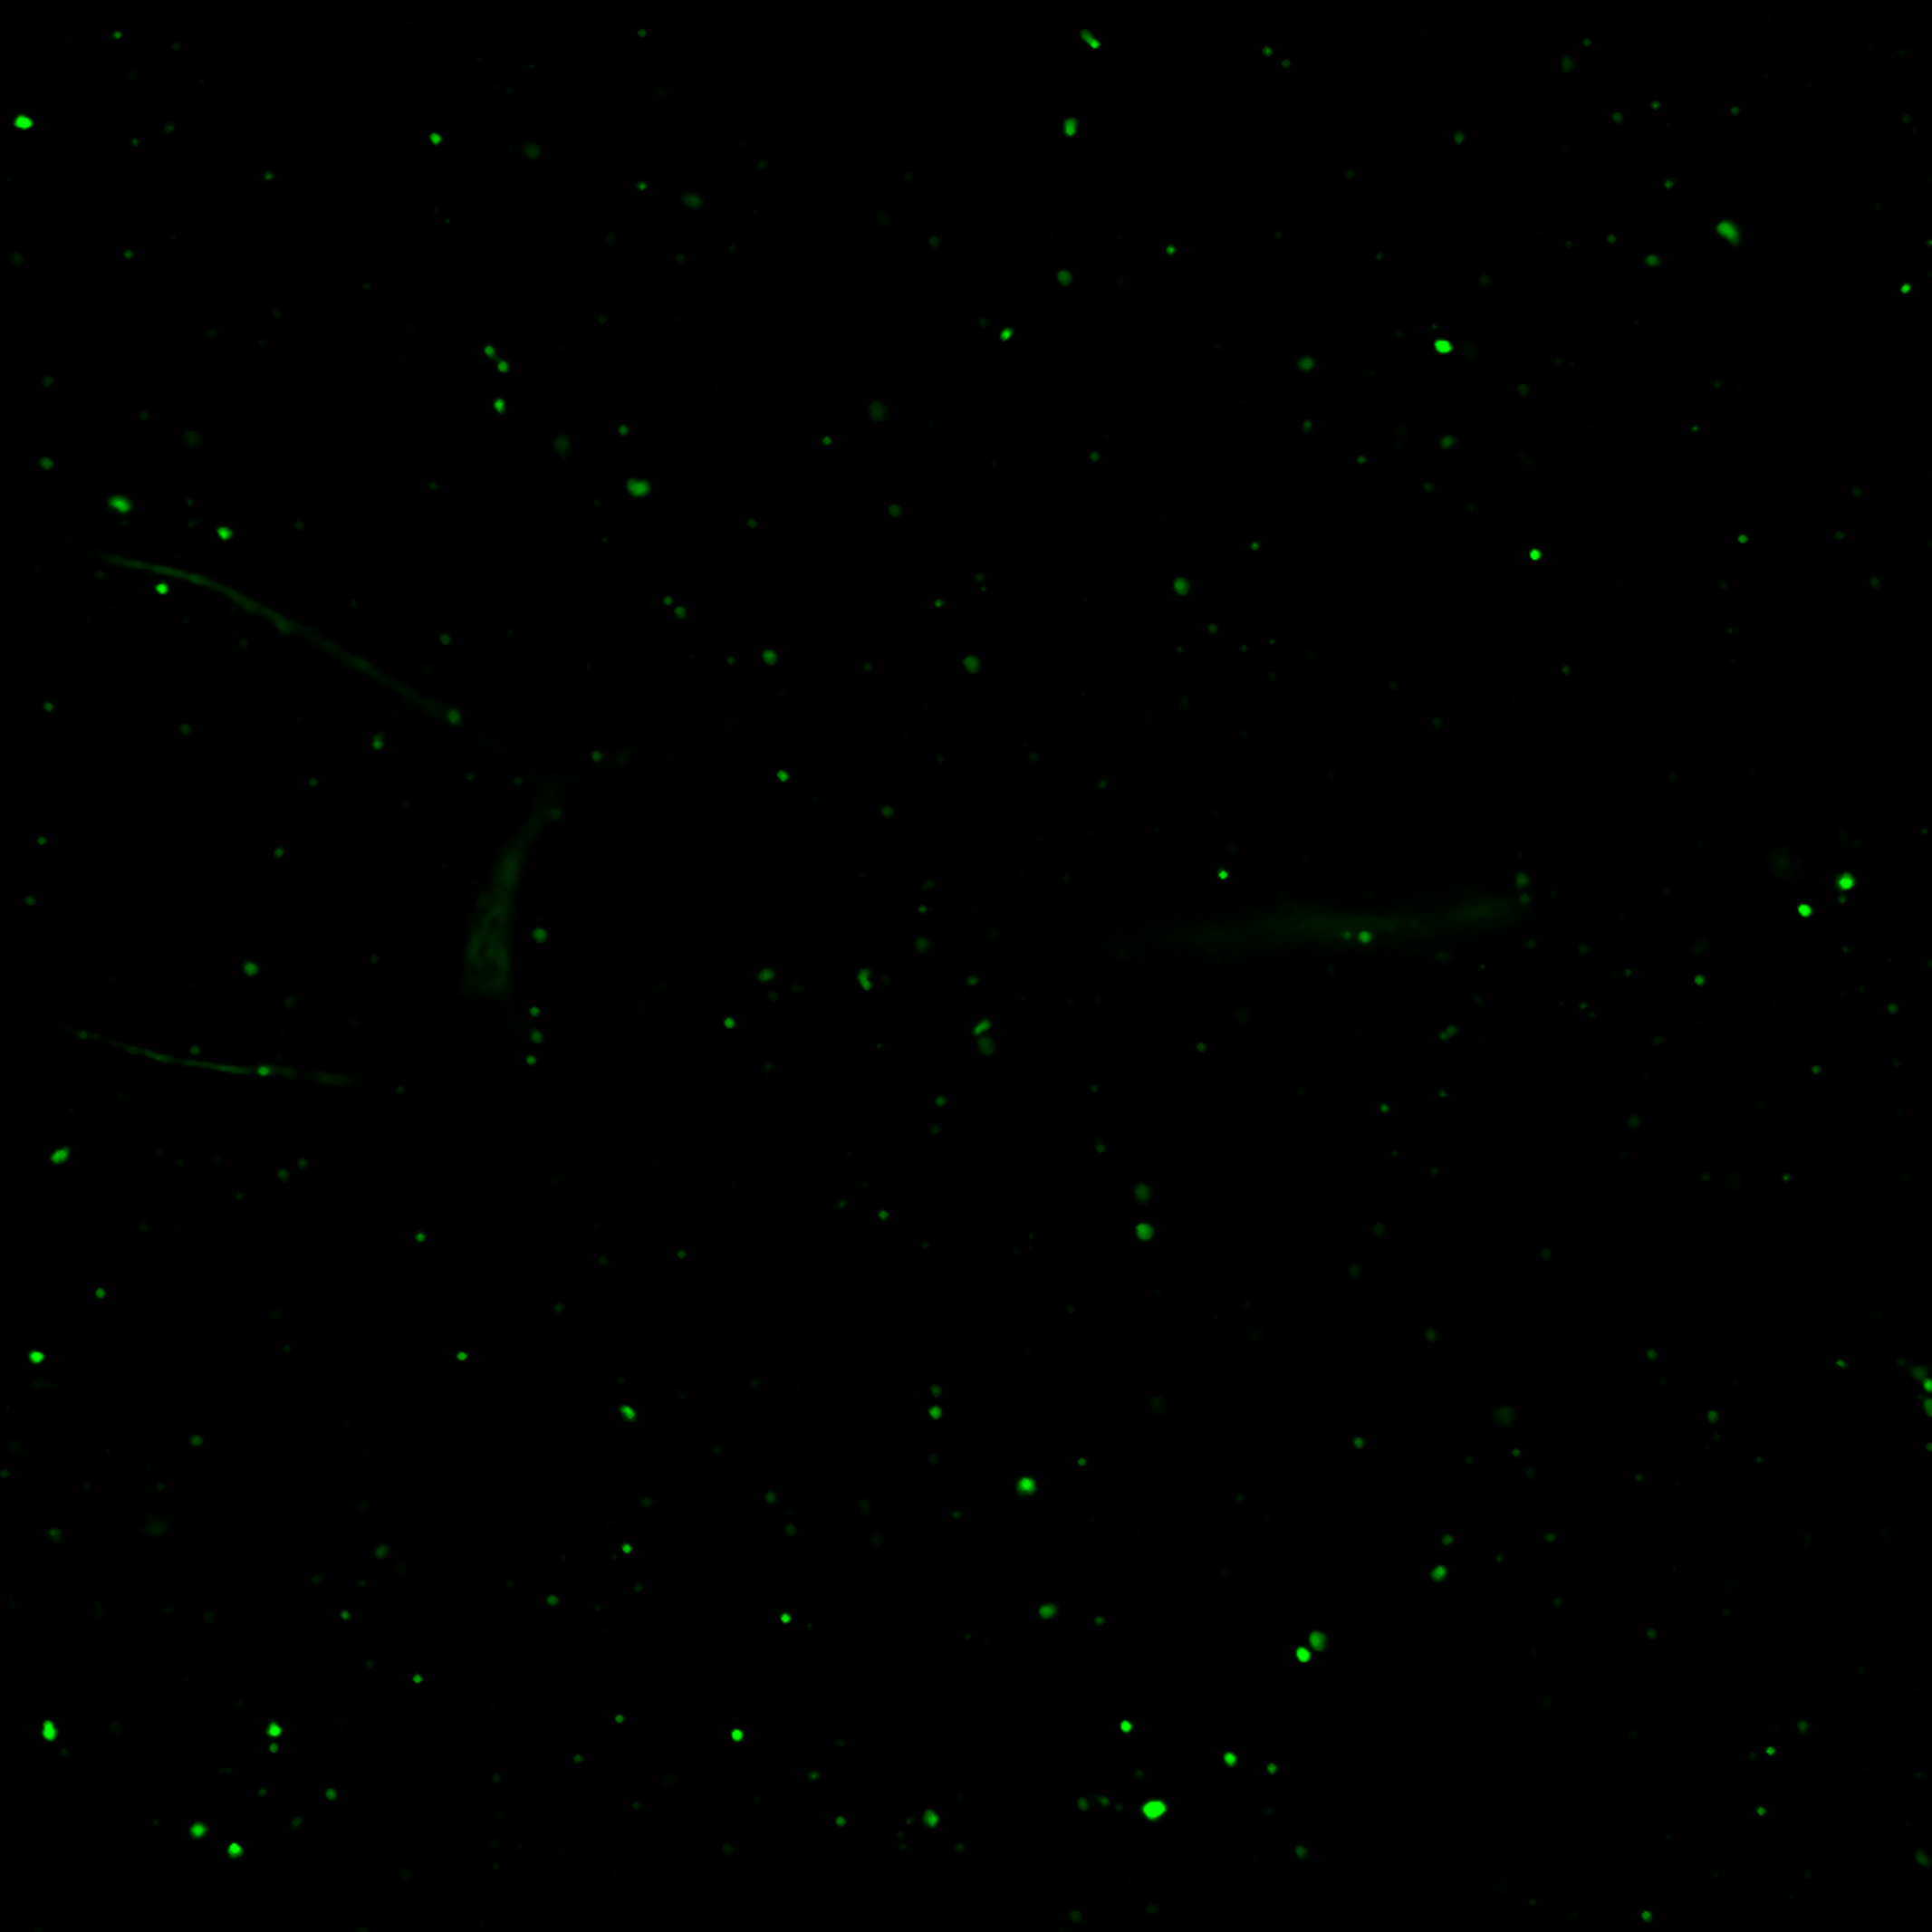
\includegraphics[height=4cm]{figure/neuron_image5}
\end{array}
$
\end{center}
\caption{\label{fig:Z-stack-images} A few of the raw images taken from Zeiss LSM 510 confocal microscope that were used in our model. The scale bar in the top left image represents 50$\mu$m and applies to all images.} 
\end{figure}
%

The confocal images were converted to a 3D voxelated data set using \textit{ImageJ} \citep{Schneider:2012dw}, where each voxel has dimensions of 0.22$\mu$m $\times$ 0.22$\mu$m $\times$ 2$\mu$m. Subsequently, the discrete geometry generated from the voxelated neuron-in-gel data was enclosed in a box that represents the domain of the collagen gel, where the neuron-gel interface is perfectly bonded. A mesh of 82,105 tetrahedral elements was generated on the non-manifold neuron-in-gel geometry using the SimModeler tool of Simmetrix Inc. \citep{simmetrix,Shephard:2000vc}. The neuron-in-gel voxelated data, discrete geometry, and corresponding mesh are shown in Figs.\ \ref{fig:image_to_model}(a) - (c), respectively. 
%
% (a) Schematic of image stack - images from N2P30/Neuron/sample2 folder. 
% (b) Neuron-in-gel model. Image generated by simModeler.
% (c) Neuron-in-gel mesh. Image generated by Paraview. N2P178/3-Neuron_FT
\begin{figure}[ht]
\begin{center}
$
\begin{array}{ccc}
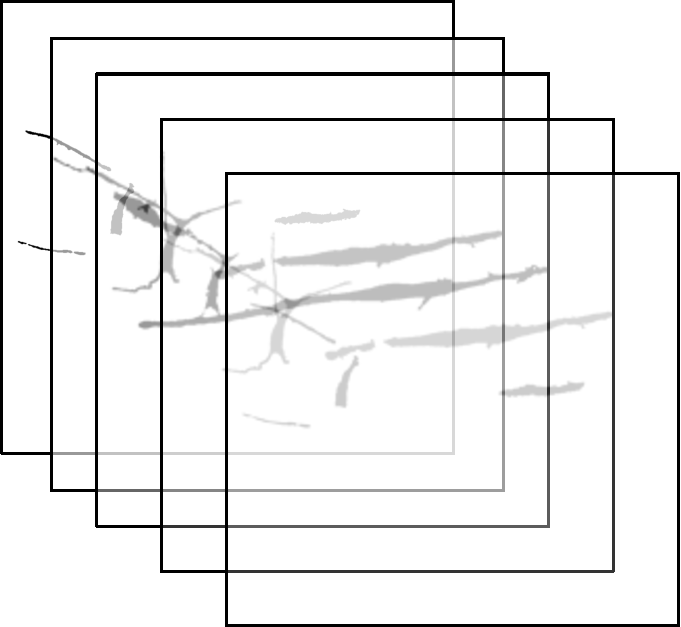
\includegraphics[height=2.5cm]{figure/ImageStack.pdf} & 
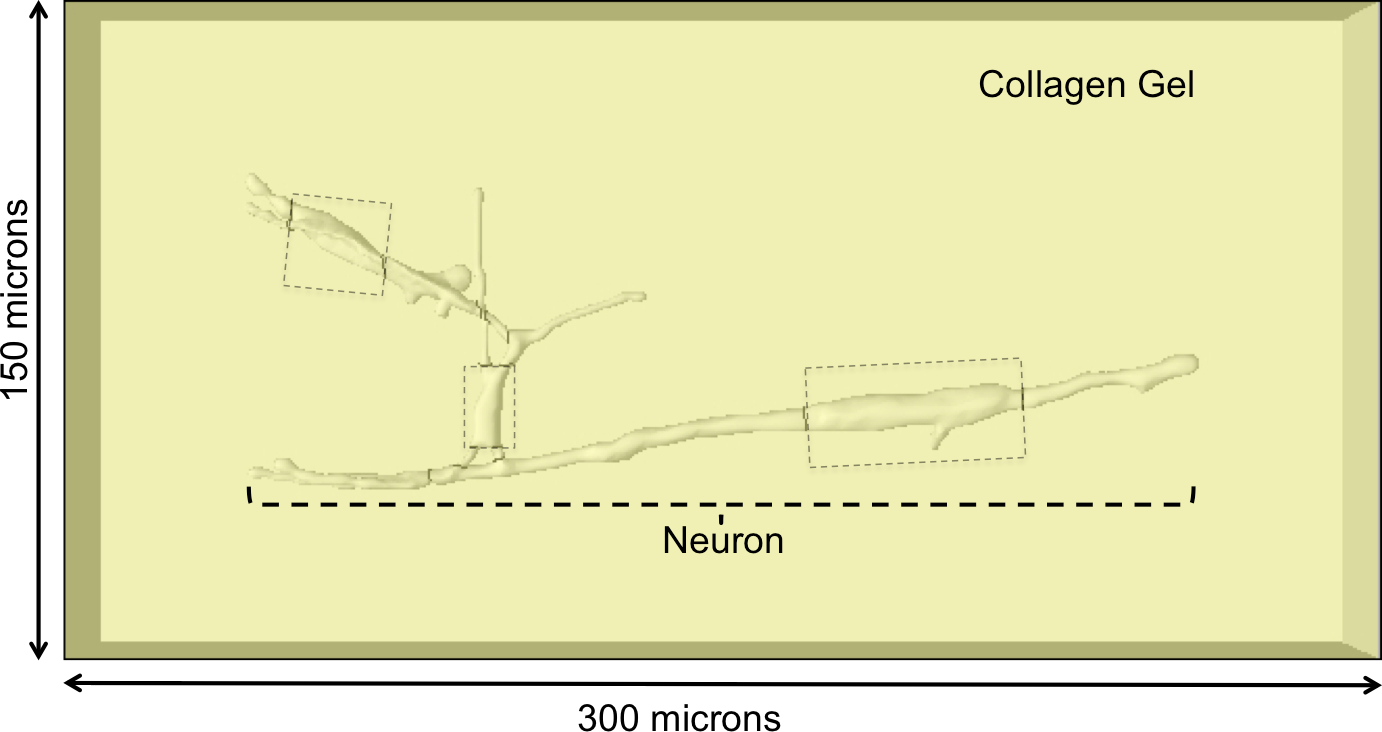
\includegraphics[height=2.5cm]{figure/neuron-in-gel_labels.pdf} &
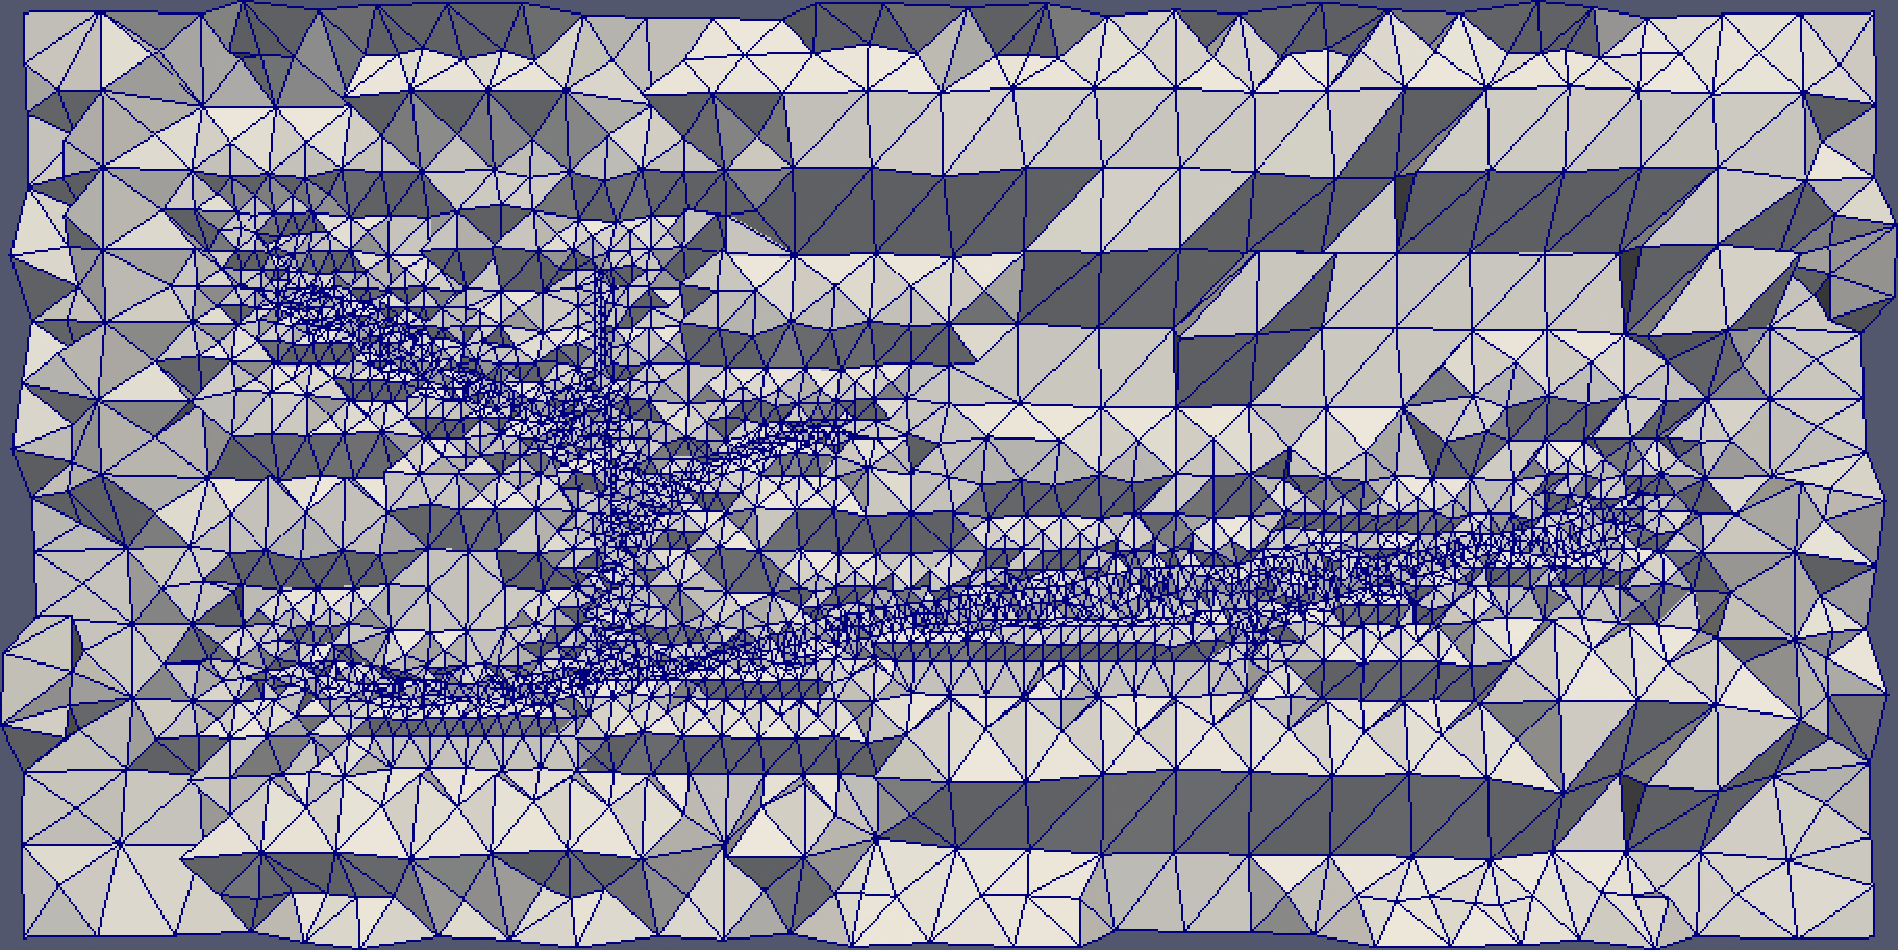
\includegraphics[height=2.5cm]{figure/neuron-in-gel_mesh.pdf} \\
(a) & (b) & (c)
\end{array}
$
\end{center}
\caption{\label{fig:image_to_model} (a) Stack of confocal images of neurons from Fig.\ \ref{fig:Z-stack-images}. (b) Geometric  model of neurons that are embedded in collagen gel. The neuron cell bodies are labeled with their axial length - axons are unlabeled. The region enclosing the neurons is the collagen gel. (c) Cut in neuron-in-gel model showing the generated mesh.}
\end{figure}
%

%%%%%%%%%%%%%%%%%%%%%%%%%%%%%%%%%%%%%%%%%%%%%%%%%%%%%%%%%%%%%%%%%%%%%%
\section{Multi-Scale Method for Modeling Collagen Gel}
\label{sec:multi-scale_method}
Collagen gels have been modeled in the past using a multi-scale formulation based on volume averaging of fiber-network representative volume elements (RVEs) \citep{Chandran:2007hy,Stylianopoulos:2007dp,Barocas:2007gk,Lai:2012ji,Lake:2012jm}. Such a multi-scale formulation is also employed in this study to model the collagen gel surrounding the neurons. The multi-scale formulation consists of two scales: the collagen-network scale that represents the fiber level and the macroscopic scale that represents the tissue level. Quantities corresponding to the collagen-network (or microscopic) and macroscopic scales are denoted with $(m)$ and $(M)$ superscripts, respectively. 

The collagen-network scale is represented by a fiber network, which defines the RVE. Each RVE is generated from the Delaunay triangulation of randomly placed seed points - the edges of the triangulation represent the fibers of the network. Each fiber only carries an axial load with the axial forces in tension and compression given by: 
%
\begin{equation}
T^{(m)} =
\begin{cases}
\frac{E_f A_f}{B} \left[ \exp(0.5 B(\lambda_f^2 - 1)) - 1\right] & \text{if } \lambda_f \le \lambda_S \\
H_S \lambda_f + h_S & \text{if } \lambda_f > \lambda_S
\end{cases}
\label{eq:fiber_force_axial}
\end{equation}
%
and
%
\begin{equation}
T^{(m)} =
\begin{cases}
\frac{E_f A_f}{B} \left[ \exp(0.5 B(\lambda_f^2 - 1)) - 1\right] & \text{if } \lambda_f \ge \lambda_C \\
H_C  \lambda_f + h_C & \text{if } \lambda_f < \lambda_C 
\end{cases},
\label{eq:fiber_force_compression}
\end{equation}
%
respectively, where 
%
\begin{align*}
&E_f: \text{linear modulus of a collagen fiber.} \\
&A_f: \text{cross-sectional area of fiber.} \\
&B: \text{constant parameter that controls nonlinearity.} \\
&\lambda_f \equiv \frac{l}{l_0} \text{ where } l \text{ and } l_0 \text{ are the current and initial lengths, respectively, of the fiber. } \\
&\lambda_S: \text{ fiber stretch value at which the fiber relation transitions from nonlinear to linear.} \\
&\lambda_C: \text{ fiber compression value at which the fiber relationship transitions from nonlinear to linear.} \\
&H_n \equiv E_f A_f\lambda_n \exp(0.5B(\lambda_n^2 - 1)) \text{ for } n=S \text{ or } C.\nonumber\\
&h_n \equiv \frac{E_f A_f}{B}\left[\exp(0.5 B (\lambda_n^2-1))-1\right] -H_n \lambda_n \text{ for } n=S \text{ or } C. 
\end{align*}
%

The fiber force in tension shown in Eq.\ \eqref{eq:fiber_force_axial} transitions from a nonlinear to linear relationship when the fiber is stretched beyond $\lambda_S$, while the fiber force in compression in Eq.\ \eqref{eq:fiber_force_compression} transitions from a nonlinear to linear relationship when the fiber is compressed below $\lambda_C$. The transition to a linear fiber force relationship for large fiber stretch in tension is consistent with experimental measurements of single collagen fibers \citep{Eppell:2006hh,Svensson:2010fr}. 

Displacement boundary conditions are imposed in order to solve for network equilibrium in the RVE. The displacements at the corners of the RVE are dictated by the deformation state of the macroscopic scale via
%
\begin{equation}
u^{(c,m)}_i = (F^{(M)}_{ij} - \delta_{ij}) \frac{x^{(c,m)}_j}{L^{(m)}},
\label{eq:downscaling}
\end{equation}
%
where $F^{(M)}_{ij}$ is the deformation gradient tensor of the macroscopic scale, $u^{(c,m)}$ are the displacements at the corners of the RVE,  and $x^{(c,m)}/L^{(m)}$ are the coordinates of the corners of the RVE. In Eq.\ \eqref{eq:downscaling}, $x^{(c,m)}_j$ are coordinates of a dimensionless computational domain that is a cube spanning the domain defined by (-0.5,0.5) in each of the coordinate axes. The scale conversion, $1/L^{(m)}$, relates the unit lengths between the computational and physical domains. It is important to note that Eq.\ \eqref{eq:downscaling} is valid because the center of the RVE is defined at the origin of the computational domain. The boundary displacements on each node lying on the boundary of the RVE are determined via linear interpolation. 

Upon solving for network equilibrium in each RVE, the volume-averaged Cauchy stress tensor of the collagen-network scale is computed from the forces acting on nodes that lie on the boundary of the RVE (bcl) \citep{Chandran:2007hy,Stylianopoulos:2007dp}
%
\begin{equation}
s_{ij}^{(m)} = \frac{1}{V^{(m)}} \sum_{\text{bcl}} x_i^{(m)} T_j^{(m)} ,
\label{eq:micro_stress_discrete}
\end{equation}
%
where $V^{(m)}$ is the current volume of the RVE, $T_j^{(m)}$ is the $j^{th}$ component of the fiber force, and $s_{ij}^{(m)}$ are elements of the microscopic stress tensor. The macroscopic Cauchy stress tensor is determined from scaling $s_{ij}^{(m)}$ by  $L^{(m)}$:
%
\begin{equation}
\sigma_{ij}^{(M)} = s_{ij}^{(m)}\left(\frac{1}{L^{(m)}}\right)^2.
\label{eq:macro_stress_discrete}
\end{equation}
%
This is needed due to the difference in length scales between the physical macroscopic domain and the non dimensional microscopic computational domain. The Cauchy stress tensor of Eq.\ \eqref{eq:macro_stress_discrete} is used to solve the macroscopic force balance \citep{Chandran:2007hy,Stylianopoulos:2007dp}
%
\begin{equation}
\sigma_{ij,i}^{(M)} = \frac{1}{V^{(m)}} \int_{\partial V^{(m)}} \left( s_{ij}^{(m)} - \sigma_{ij}^{(M)} \right)u_{k,i}^{(m)} n_k dA^{(m)},
\label{eq:macro_stress_divergence}
\end{equation}
%
where $u_k^{(m)}$ is the displacement of the RVE boundary on the microscale and $n_k$ is the unit normal vector. The right-hand side of Eq.\ \eqref{eq:macro_stress_divergence} acts as a body force that accounts for the correlation between the inhomogeneous displacement of the RVE boundary and local inhomogeneities in the stress field�\citep{Chandran:2007hy,Stylianopoulos:2007dp}. Equation \eqref{eq:macro_stress_divergence} arises from integration of the microscopic-scale (RVE) Cauchy stress balance, $\sigma_{ij,i}^{(m)} = 0$. If the RVE did not deform, then the averaged equation would just be $\sigma^{(M)}_{ij,i}=0$. When the RVE deforms, however, and that deformation is position-dependent, then the average of the divergence of the stress ($\sigma_{ij,i}^{(m)}$) is no longer equal to the divergence of the average stress ($\sigma_{ij,i}^{(M)}$), and a correction term must be introduced, analogous to the corresponding term in the Reynolds transport theorem \citep{Whitaker-1999}. This is expressed by the right-hand side of Eq.\ \eqref{eq:macro_stress_divergence} and accounts for the correlation between RVE stress and boundary displacement.

The scaling parameter between the computational and physical domains, $L$, in Eqs.\ \eqref{eq:downscaling} and \eqref{eq:macro_stress_discrete} is required for both the downscaling and upscaling procedures. It is determined by comparing the average fiber length in the RVEs to that of the fiber network in 2 mg/mL collagen gel used in \citep{Zhang:2016ga}. The mean fiber length in such a network is 1.81 $\mu$m \citep{Lindstrom:2013gd}.

%%%%%%%%%%%%%%%%%%%%%%%%%%%%%%%%%%%%%%%%%%%%%%%%%%%%%%%%%%%%%%%%%%%%%%
\section{Constitutive Relationship for Modeling of Neurons}
Cross-linked axially-aligned microtubule bundles are a major structural feature of axons and give rise to macroscopic anisotropic mechanical behavior \citep{Peter:2012fc}. To account for such mechanical anisotropy, the axons are modeled as a transversely isotropic hyperelastic material \citep{JavierBonet:2008uxa,Bonet:1998vc}. The elements of the Cauchy stress tensor and spatial (Eulerian) elasticity tensor are expressed in terms of neo-Hookean (nh) and transversely isotropic (trns) components \citep{Bonet:1998vc}
%
\begin{equation}
\sigma_{ij} = \sigma^{\text{nh}}_{ij} + \sigma^{\text{trns}}_{ij} \ \ \text{ and } \ \ c_{ijkl} = c^{\text{nh}}_{ijkl} + c^{\text{trns}}_{ijkl},
\end{equation}
%
respectively, where 
%
\begin{align}
&\sigma^{\text{nh}}_{ij} = \frac{\mu}{J}(b_{ij} - \delta_{ij}) + \lambda(J-1)\delta_{ij} \nonumber\\
%
&\sigma^{\text{trns}}_{ij} = \frac{2\beta}{J}(a_r a_r - 1)\delta_{ij} + \frac{2}{J}[\alpha+2\beta\ln J+2\gamma(a_r a_r -1)]a_i a_j - \frac{\alpha}{J}(b_{is}a_s a_j+a_i b_{jr}a_r) \nonumber\\
%
&c^{\text{nh}}_{ijkl} = \lambda(2J-1)\delta_{ij}\delta_{kl} + \frac{2}{J}[\mu - \lambda J(2J-1)]\delta_{ik}\delta_{jl} \nonumber\\
%
&c^{\text{trns}}_{ijkl} = \frac{8\gamma}{J}a_i a_j a_k a_l + \frac{4\beta}{J}(a_i a_j \delta_{kl} + \delta_{ij}a_k a_l) - \frac{\alpha}{J}(a_i a_l b_{jk} + b_{ik}a_j a_l) - \frac{4\beta}{J}(a_r a_r - 1)\delta_{ik}\delta_{jl}.
\label{eq:trns_iso}
\end{align}
%
In Eq.\ \eqref{eq:trns_iso}, $b_{ij}$ are elements of the left Cauchy-Green strain tensor and $a_i$ is a component of the mapping of the direction of anisotropy in the undeformed state to the current state via the deformation gradient. In tensor notation, $\pmb{a} \equiv \pmb{F}\pmb{A}$, where $\pmb{A}$ is the direction of aniostropy in the undeformed state and $\pmb{F}$ is the deformation gradient tensor. $\lambda$ and $\mu$ are the Lam\'e constants that define the material properties of the isotropic component, while $\beta$, $\gamma$, and $\alpha$ are parameters that define the material properties of the anisotropic component. The parameters of Eq.\ \eqref{eq:trns_iso} can be written in terms of material constants as
%
\begin{align}
&\lambda = \frac{2\mu (\nu+n\nu^2)}{m} \ \ \ \ \ \gamma = \frac{E_A(1-\nu)}{8m} - \frac{\lambda+2\mu}{8} + \frac{\alpha}{2} - \beta \nonumber\\
%
&\alpha = \mu - G_A \ \ \ \ \ \ \ \ \ \ \ \ \ \ m = 1 - \nu - 2 n\nu^2 \nonumber\\
%
&\beta = \frac{\mu \nu^2(1-n)}{2m} \ \ \ \ \ \ \ \ n = \frac{E_A}{2\mu(1+\nu)},
\label{eq:trns_iso_constants}
\end{align}
%
where $\mu$ is the shear modulus, $G_A$ is the axial shear modulus, $\nu$ is the Poisson ratio, and $E_A$ is axial Young's modulus. In our analysis, the shear modulus is set to be isotropic such that $G_A=\mu$ and $\alpha = 0$. All the constants in Eq.\ \eqref{eq:trns_iso_constants} are set once all material constants ($\mu$, $G_A$, $\nu$, and $E_A$) are specified. 

%%%%%%%%%%%%%%%%%%%%%%%%%%%%%%%%%%%%%%%%%%%%%%%%%%%%%%%%%%%%%%%%%%%%%%
\section{Parameter Specifications}

\subsection{Parameters of Collagen Network}

The parameters for the collagen network are listed in Table \ref{table:multi-scale_parameters}.
%%%%%%%%%%%%%%%%%%%%%%%%%%%%%%%%%%%%%%%%%%%%%%%%%%%%%%%%
\begin{table}[ht]
\begin{center}
\begin{tabular}{ l c l }
\hline \hline
Parameter & Specification & Source \\
\hline 
$E_f$ & 200 kPa & Fit to experimental data. \\
$A_f$ & 82.5 $\mu$m$^2$ & Based on \cite{Dutov:2016gu} \\
$B$ & 20 & Fit to experimental data. \\
$\lambda_S$ &1.13 & Fit to experimental data. \\
$\lambda_C$ & 1.0 & Selected. \\ 
$H_S$ & 297.25 $\mu$N & From above parameters.\\
$H_C$ & 16.5$\mu$N & From above parameters. \\
$h_S$ & -322.74 $\mu$N & From above parameters. \\
$h_C$ & -15.67$\mu$N & From above parameters. \\
$L^{(m)}$ & 7 $\mu$m & Based on \cite{Lindstrom:2013gd}. See Section \ref{sec:multi-scale_method}.\\ 
\hline \hline
\end{tabular}
\end{center}
\caption{Parameters for multi-scale model of collagen gel.}
\label{table:multi-scale_parameters}
\end{table}
%%%%%%%%%%%%%%%%%%%%%%%%%%%%%%%%%%%%%%%%%%%%%%%%%%%%%%%%
These values were chosen to obtain a good fit to experimental engineering stress-strain curves. To obtain the stress-strain responses experimentally, collagen I gels identical to those embedding the neurons were subjected to uniaxial tensile loading at 0.5mm/s up to 25$\%$ strain using an Instron 5865 (Instron, Norwood, MA), as described in  \cite{Zhang:2016ga}. The Instron Bluehill software collected the force and displacement data at 1kHz during loading. 

As seen in Fig.\ \ref{fig:multi-scale_properties}(b), a good fit to the stress-strain curve was obtained using the parameters listed in Table \ref{table:multi-scale_parameters}. The value of $A_f$ was chosen according to Ref.\ \citenum{Dutov:2016gu} where the fiber radius of rat tail collagen I was measured to be 162 nm. The parameters $E_f$ and $B$ were adjusted to capture the stiffening in the stress-strain curve that arises at approximately 11$\%$ strain, while $\lambda_S$ was adjusted to capture the stiffness of the linear regime in the stress-strain curve at large strains. In principle, fibers do not carry load in compression. Since the fibers in this model only have axial forces, the value of $\lambda_C$ was selected to give a stiffness in compression that is significantly smaller than that in tension. The fiber-force curve for the parameters listed in Table \ref{table:multi-scale_parameters} is plotted in Fig.\ \ref{fig:multi-scale_properties}(b) where the stiffness in tension and compression in the linear regimes of the fiber force are 29.7 kPa and 1.65 kPa, respectively.
%
% (a) fiber force curve from N2P177/LRT_Compression folder.
% (b) stress-strain curve from N2P178/1-NewParams_Cube/stress-strain folder.
% (c) Poisson ratio curve from N2P178/1-NewParams_Cube/poisson-ratio folder.
% (d) Alignment curve from N2P178/1-NewParams_Cube/alignment folder.
\begin{figure}[ht]
\begin{center}
$
\begin{array}{cc}
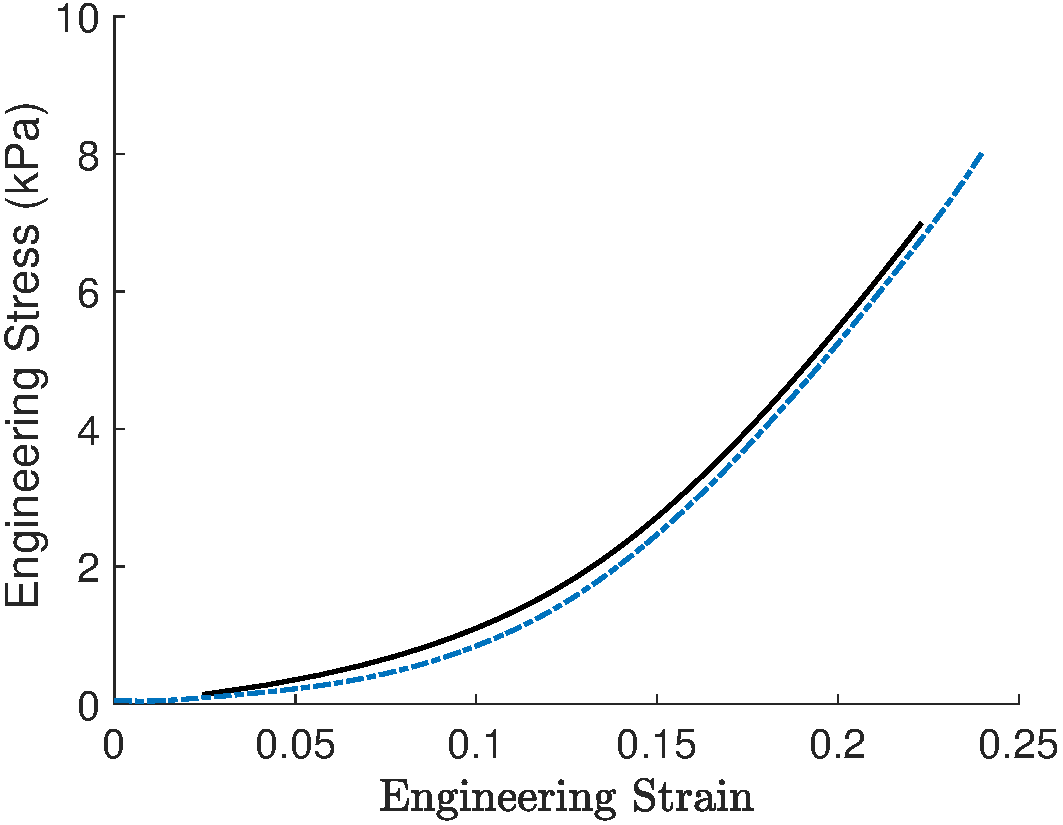
\includegraphics[height=5cm]{figure/stress_strain.pdf} &
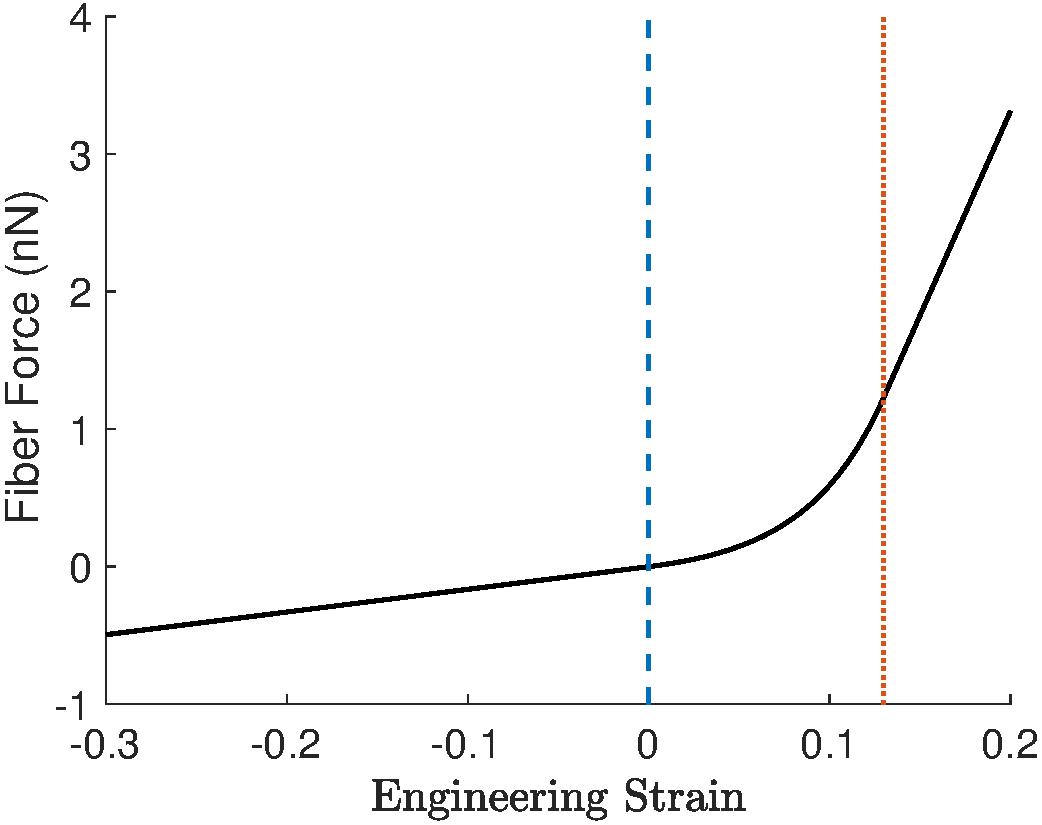
\includegraphics[height=5cm]{figure/FiberForceRelation.pdf} \\
(a) & (b) 
\end{array}
$
\end{center}
\caption{\label{fig:multi-scale_properties} Plots of (a) stress-strain curve and (b) fiber force for parameters listed in Table \ref{table:multi-scale_parameters}. Results from simulation plotted using black solid line, while experimentally measured data is plotted in blue dash-dotted line.}
\end{figure}
%

For the parameters in Table \ref{table:multi-scale_parameters}, fiber alignment was also examined. Fiber alignment is measured using the orientation index $P_2$. The value of $P_2$ is calculated from the angle $\theta$ between fibers and the direction of stretch
%
\begin{equation}
P_2 = \frac{3 <\cos^2\theta> - 1}{2},
\label{eq:P2_simulation}
\end{equation}
%
where $<x>$ denotes the average of $x$ over all fibers. The value of $P_2$ ranges from 1 in which the fibers are completely aligned to -1/2 in which all fibers are orthogonal to the alignment direction. When $P_2=0$, the fiber network is randomly oriented. 

Experimentally, the fiber alignment in innervated collagenous tissue was measured using the Quantitative Polarized Light Imaging (QPLI) method \citep{Quinn:2008df,Quinn:2009bf} where alignment angle $\alpha$ and retardation $\delta$ were measured in each pixel. The customized QPLI system \citep{Zhang:2016ga} is comprised of a fiber-optic light source (Dolan-Jenner Industries Inc., Boxborough, MA), a motor-controlled linear polarizer (Edmund Optics, Barrington, NJ) that rotates at 750 rpm, and a circular analyzer mounted to a high-speed camera (Phantom-v9.1; Vision Research Inc, Wayne, NJ) \citep{Zhang:2016ga}. The QPLI system was integrated with the mechanical testing device, and collagen I gels were placed between the rotating polarizer and the circular analyzer. Polarized light images were acquired during tensile loading at 500 fps with 14.5 pixel/mm resolution and processed using harmonic analysis to extract the alignment angle and retardation \citep{Tower:2002hk,Quinn:2008df}. The orientation index $P_2$ is calculated from $\alpha$ and $\delta$ of the QPLI method via (see Appendix A for derivation)
%
\begin{align}
&P_2 = \frac{1}{2}\left(3 \int_0^{\pi} p(\theta) \cos^2\theta d\theta - 1\right) \nonumber\\
&p(\theta) = \frac{1}{N} \sum_{i=1}^N \left[ \frac{1-2\delta_i}{\pi} + \frac{4 \delta_i}{\pi}\cos^2(\theta - \alpha_i)\right],
\label{eq:P2_experiment}
\end{align}
%
where $\delta_i$ and $\alpha_i$ are the retardation and alignment angle, respectively, of the $i^{th}$ pixel. The probability distribution, $p(\theta)$, is a convenient approximation of the actual distribution of collagen orientation in the sample. The fiber alignment as a function of applied grip strain calculated from simulation and measured experimentally are plotted in Fig.\ \ref{fig:fiber_alignment} where the general trend in alignment behavior is in agreement. 
%
%  Alignment curve from N2P178/1-NewParams_Cube/alignment folder.
\begin{figure}[ht]
\begin{center}
$
\begin{array}{c}
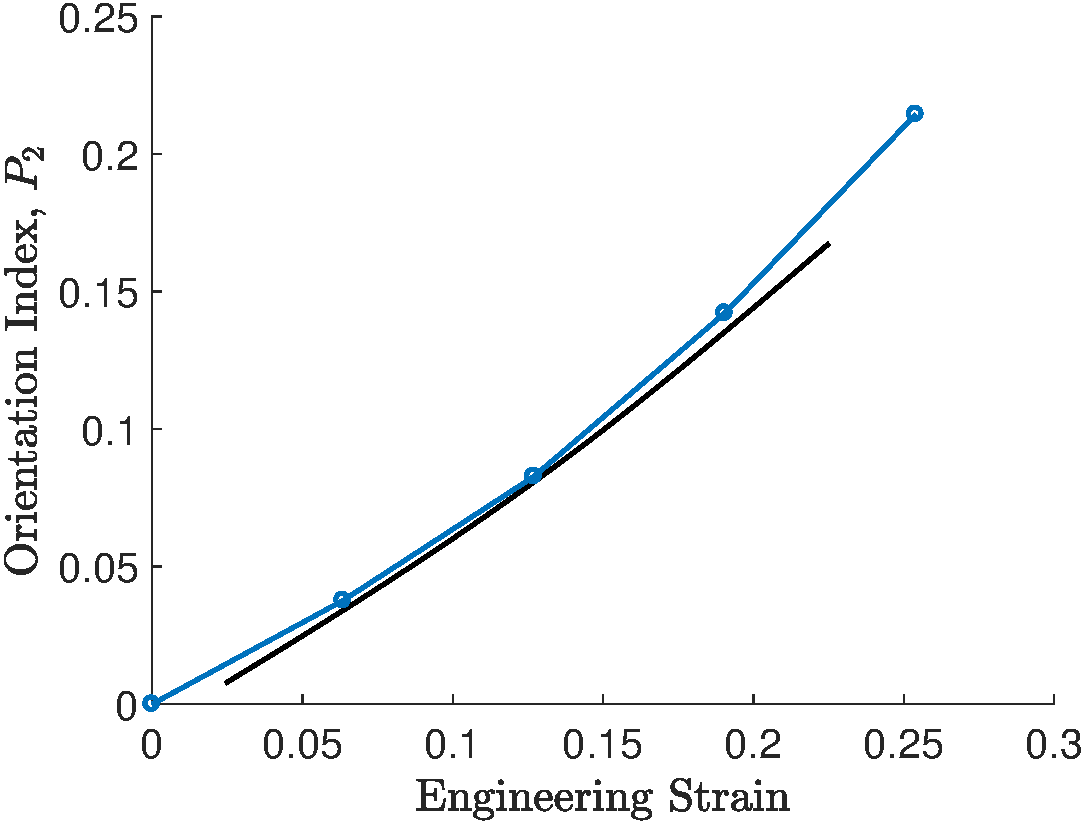
\includegraphics[height=5cm]{figure/alignment.pdf} 
\end{array}
$
\end{center}
\caption{\label{fig:fiber_alignment} Fiber aligment metric $P_2$ for parameters listed in Table \ref{table:multi-scale_parameters}. Results from simulation plotted using black solid line, while experimentally measured data are plotted in blue dotted line.}
\end{figure}
%
%\textcolor{red}{[According to Professor Picu, alignment is more pronounced at low strains and less pronounced at high strains if deformation is non-affine (compared to the case of affine deformation). The behavior in Fig.\ \ref{fig:fiber_param2}(b) is in agreement if it is valid that the Delaunay fiber network that we are using deforms affinely due to the the large coordinate of the Delaunay network used in our model.]}

\subsection{Parameters of the Constitutive Description of the Neurons}

The value of $E_A$ in Eq.\ \eqref{eq:trns_iso_constants} is based on the study by Peter and Mofrad \citep{Peter:2012fc}, where the mechanical behavior of axonal microtubule bundles under tension was simulated with a discrete bead-spring model. To apply their results for microtubule bundles to our neuron model, we assume that only the microtubule bundles carry force in the axon and that the stress of the microtubule bundles can be redistributed over the cross-sectional area of the axon. Since the microtubules are the stiffest component of the cytoskeleton \citep{Fletcher:2010ku}, the mechanical contribution from the actin filaments (membrane cortex) is ignored. Based on these assumptions, the axial stiffness of the axon can be related to the axial stiffness of the microtubule bundles, $E_{MTb}$, by
%
\begin{equation}
E_A = \frac{E_{MTb} A_{MTb}}{A_A},
\label{eq:EA_EMTb_relation}
\end{equation}
%
where $A_{MTb}$ and $A_A$ are the cross-sectional areas of the microtubule bundle and axon, respectively. Peter and Mofrad \citep{Peter:2012fc} suggested that the stress-strain relationship of the microtubule bundle is well represented by a power-law fit that results in a strain-dependent elastic modulus. For this study, $E_{MTb}$ was taken to be $1\times 10^5$ kPa, where the corresponding tangent stiffness is 5.8$\times 10^8$ kPa. The value of $A_{MTb}$ was determined to be 0.00933 $\mu$m${}^2$ based on the diameter of each microtubule and the number of microtubule cross sections within a microtubule bundle, see Ref.\ \citep{Peter:2012fc} for schematic. We assume that the cross-section of the microtubule bundle contains 19 rows of microtubules, each with a diameter of 25 nm. Lastly, the value of $A_A$ was determined to be 13.3 $\mu$m${}^2$, based on an average axon diameter of approximately 4 $\mu$m in the neuron. From the above values, $E_A$ is determined from Eq.\ \eqref{eq:EA_EMTb_relation} to be 70 kPa. 

The parameters used in Eq.\ \eqref{eq:trns_iso_constants} for modeling the neuron structure are listed in Table \ref{table:neuron_parameters}. 
%%%%%%%%%%%%%%%%%%%%%%%%%%%%%%%%%%%%%%%%%%%%%%%%%%%%%%%%
\begin{table}[ht]
\begin{center}
\begin{tabular}{ l c l }
\hline \hline
Parameter & Specification & Source\\
 \hline
$E_A $ & 70 kPa & Calculated from Eq.\ \eqref{eq:EA_EMTb_relation}. \\ 
$E_T $ & 1.5 kPa & Based on \cite{Simon:2016ig} \\
$\nu $ & 0.3 & Selected. \\
$\mu $ & 0.577 kPa & Calculated from $E_T$ and $\nu$. \\ 
$G_A (= \mu) $ & 0.577 kPa & Shear modulus assumed to be isotropic.\\ 
\hline
$n $ & 46.7 & Calculated from $E_A$, $\mu$, and $\nu$. \\
$m $ & -7.7 & Calculated from $\nu$ and $n$. \\
$\lambda $ &  -0.67 kPa & Calculated from $\nu$, $\mu$, $n$, and $m$. \\
$\alpha $ & 0 kPa & Calculated from $\mu$ and $G_A$. \\
$\beta $ & 0.154 kPa & Calculated from $\mu$, $\nu$, $n$, and $m$. \\
$\gamma $ & -1.01 kPa & Calculated from $E_A$, $\nu$, $m$, $\lambda$, $\mu$, $\alpha$, and $\beta$.\\
\hline \hline
\end{tabular}
\end{center}
\caption{Parameters for constitutive model of neuron.}
\label{table:neuron_parameters}
\end{table}
%%%%%%%%%%%%%%%%%%%%%%%%%%%%%%%%%%%%%%%%%%%%%%%%%%%%%%%%
%
The transverse stiffness of the axons and cell bodies was based on the measurements of Simon et al.\ \citep{Simon:2016ig} and chosen to be 1.5 kPa. The six constants in Eq.\ \eqref{eq:trns_iso_constants} are all determined when the values listed in Table \ref{table:neuron_parameters} are fully specified.

The axial stiffness of the cell body was chosen based on the relative alignment of the microtubules. The microtubules transition from an almost perfectly aligned state in the axon to a generally unaligned state within the cell body \citep{MofradBook}. Within the cell body, the microtubules become progressively less aligned with the center of the cell body having the least alignment. Consequently, the axial stiffness within the cell body decreases and is lowest at the center. The cell bodies are modeled as a transversely isotropic hyperelastic material of axial stiffness represented by a function of position within a cell, Eq.\ \ref{eq:cellEA}. 
%
\begin{equation}
E_A^{cell} = \left(1 - \frac{D}{t}\right)E_A.
\label{eq:cellEA}
\end{equation}
%
In Eq.\ \eqref{eq:cellEA} $D$ is the distance of an interior point of the cell body to the closest axon, and $t$ is a constant describing the rate of change of $E_A^{cell}$. The geometry shown in Fig.\ \ref{fig:image_to_model}(b) indicates that the parameter $D$ ranges from 9 to 25 $\mu$m. We select a value of $t=30$ $\mu$m for our calculations. The axial stiffness of the neuron structure evaluated based on these parameters is shown in Fig.\ \ref{fig:axial_stiffness}.
%
%image for axial young's modulus from N2P178/3-Neuron_FT folder
\begin{figure}[ht]
\begin{center}
$
\begin{array}{c}
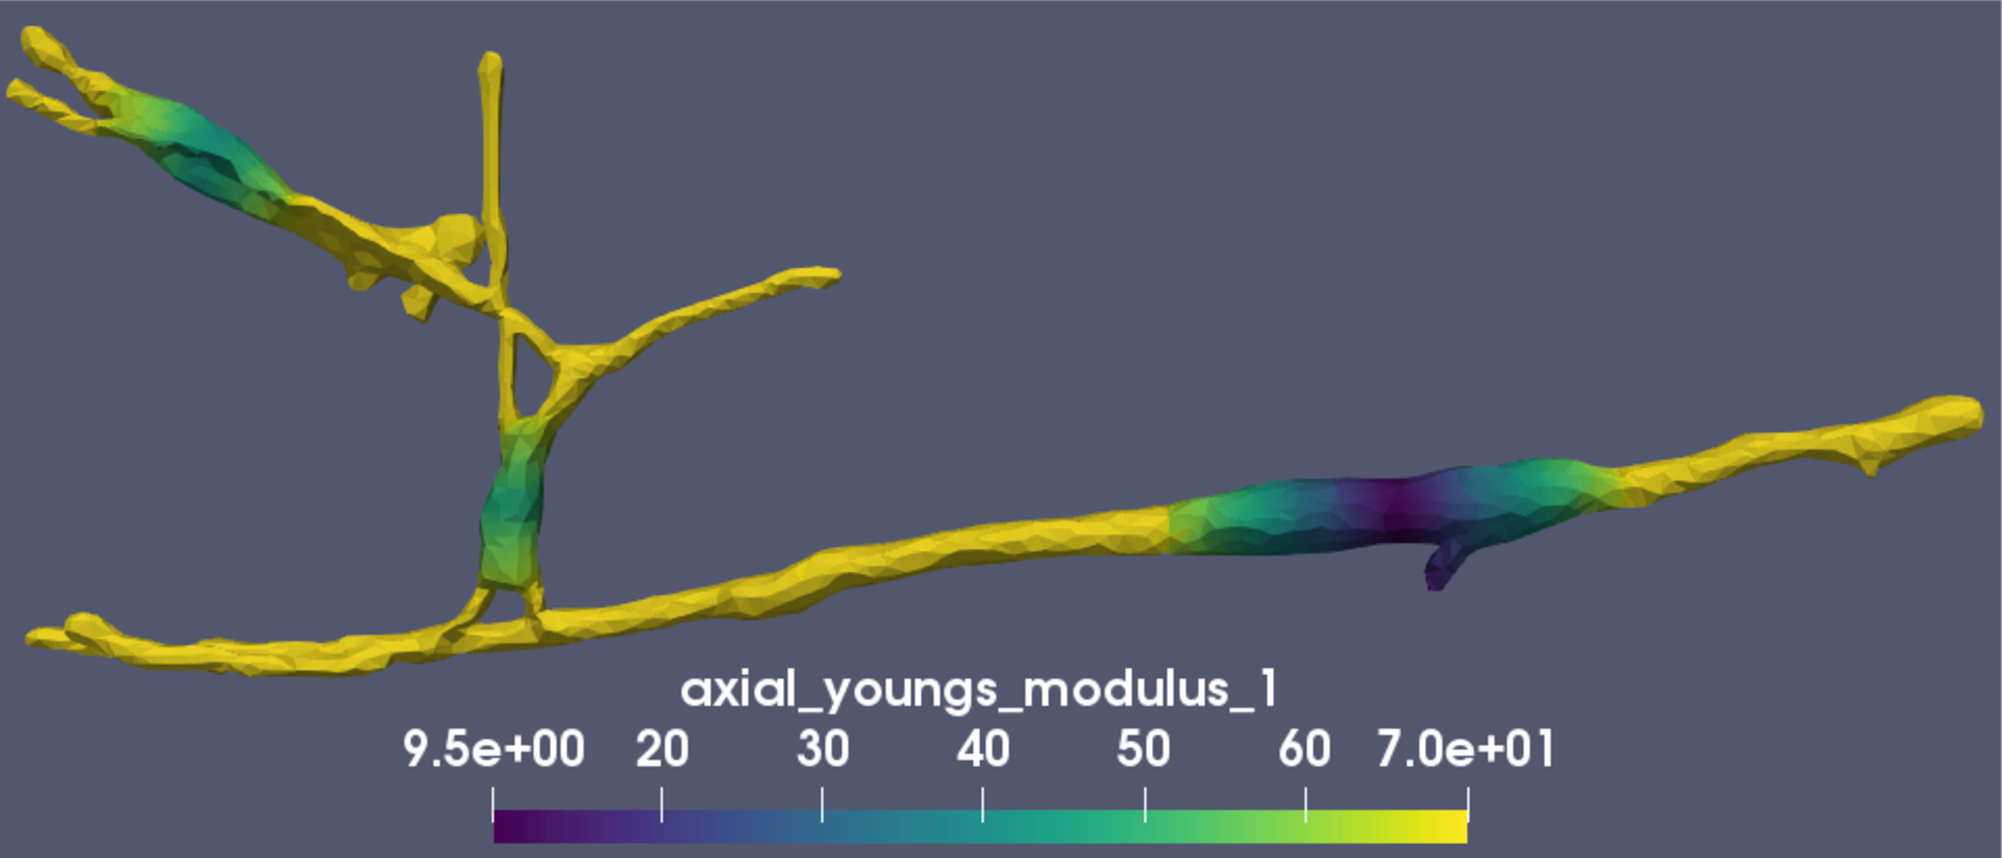
\includegraphics[height=3.5cm]{figure/axial_youngs_modulus_a30.pdf} 
\end{array}
$
\end{center}
\caption{\label{fig:axial_stiffness} Axial stiffness of neuron structure analyzed.}
\end{figure}
%

%%%%%%%%%%%%%%%%%%%%%%%%%%%%%%%%%%%%%%%%%%%%%%%%%%%%%%%%%%%%%%%%%%%%%%
\section{Implementation}
\label{sec:implementation}

%\input{figure/multi-scale-coupling-data.pdf_tex}\label{fig:coupling-data}
\subsection{Multi-scale}
Our multi-scale model is implemented using the adaptive multi-scale simulation infrastructure (AMSI) \citep{Tobin:2017ip}, which is designed to support massively parallel simulations on multiple scales. AMSI accommodates the computational demands of the multi-scale simulation by combining existing single-scale analysis codes into multi-scale analyses.

The macroscopic simulation code and the microscopic simulation codes are independent codes coupled through the AMSI libraries. AMSI manages the parallel execution space for each code, as well as the parallel communication required for the transmission of required data between them. Each of the scales in the simulation supplies information required to inform the requirements of the multi-scale communication and the distribution of inter-scale coupling data in both the parallel execution space and the problem domain. This data is used by AMSI to communicate the coupling data required at each phase of simulation, and accommodate dynamic run-time operations such as load balancing. A discussion of the underlying design considerations of AMSI can be found in \citep{Delalondre:2010kt}.

The physical scales of macroscopic continuum and the microscopic collagen network are assumed to be strongly separated allowing the application of well-defined domain relationships between the scales. Thus no runtime considerations are required with respect to domain data locality. Parallel data locality of the required coupling data must still be accounted for during simulation execution.

The macroscopic-scale domain is discretized using an unstructured mesh that is partitioned across the parallel execution space of the scale. Figure \ref{fig:scales} depicts the relationship between the two scales with respect to the macroscopic-scale unstructured mesh, an individual numerical integration point on that mesh, and the RVE-level microscopic-scale simulation corresponding to that macroscopic-scale location.
%
\begin{figure}[ht]
\begin{center}
$
\begin{array}{c}
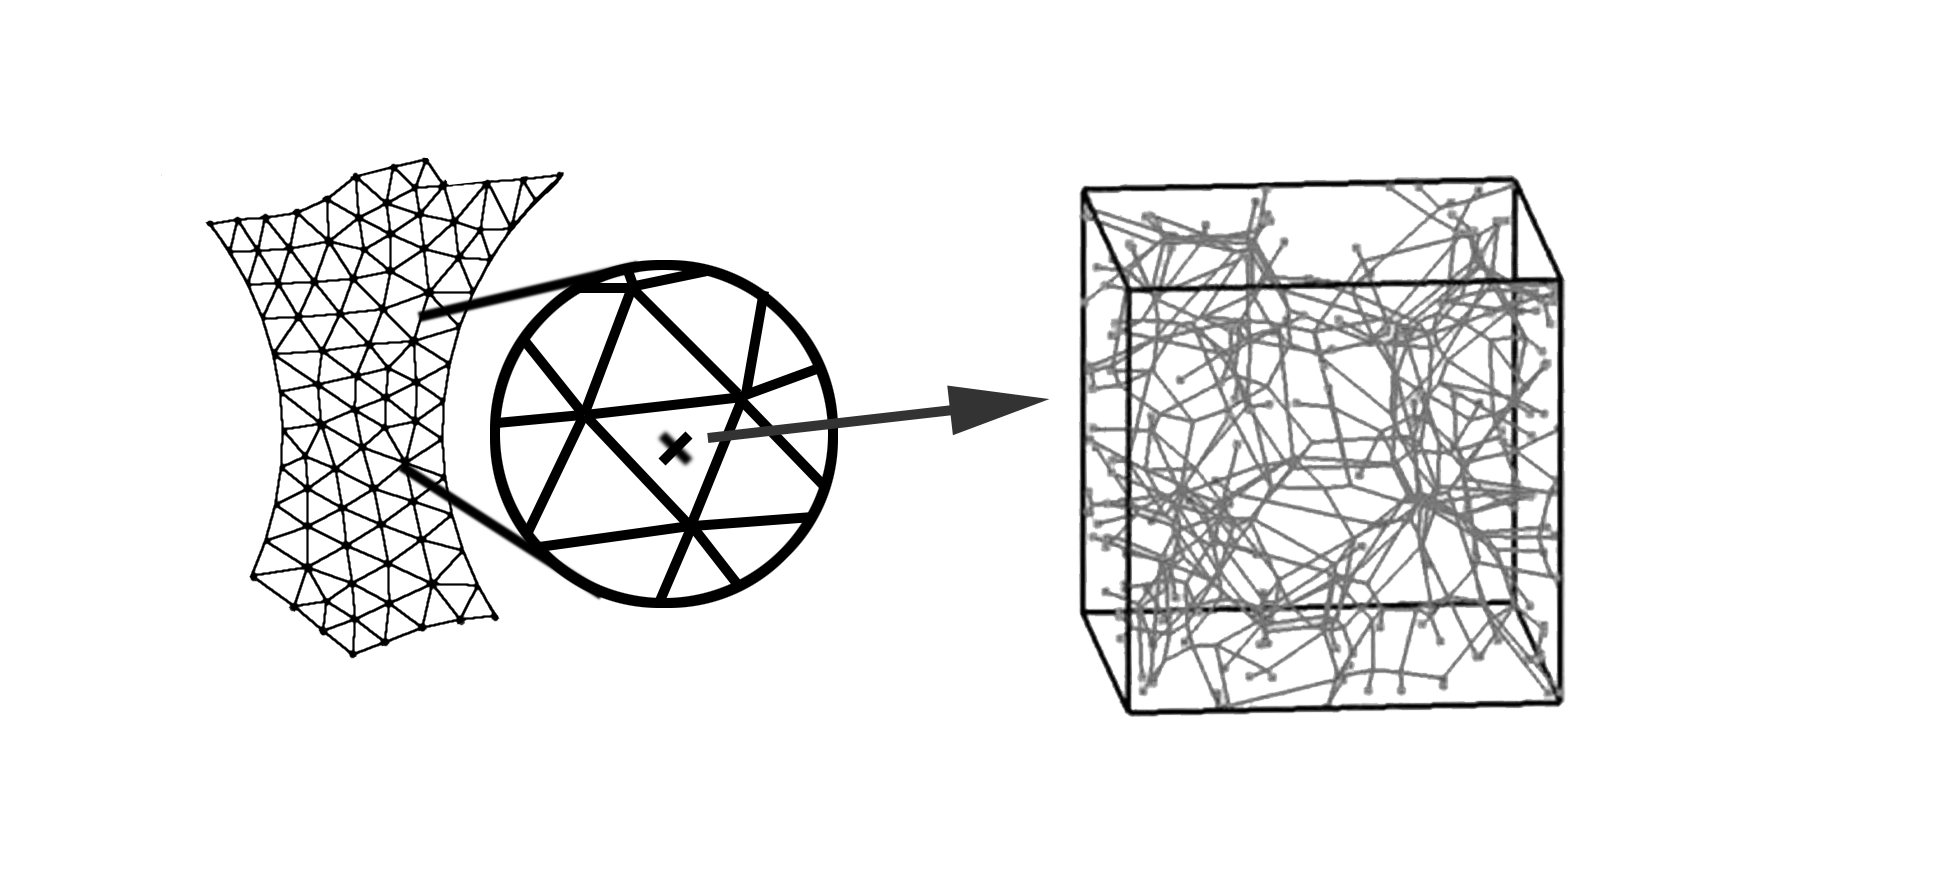
\includegraphics[height=4cm]{figure/biotissue-scales.png} 
\end{array}
$
\end{center}
\caption{\label{fig:scales} Schematic showing the hierarchy of scales in the multi-scale simulation}
\end{figure}
%

AMSI models the relationship between the domains of the macroscopic and microscopic scale problem. At each macroscopic-scale numerical integration point, the deformation gradient $\pmb{F}$ is calculated and provided to the AMSI coupling system, which uses a communication plan to provide the value to the collagen-network scale RVE simulation related to the integration point. This value is used by the collagen-network scale as shown in Eq.\ \eqref{eq:downscaling} to establish the boundary conditions for the current state of the RVE problem. Once a solution has been reached for the collagen-network scale simulation, the macroscopic-scale stress term $\sigma^{(M)}$ from Eq.\ \eqref{eq:macro_stress_discrete} and the macroscopic-scale stress divergence term $\div \sigma^{(M)}$ from Eq.\ \eqref{eq:macro_stress_divergence} are supplied to AMSI. These terms are communicated to the macroscopic scale and associated with the coupled integration point for use in assembling the macroscopic-scale linear algebraic system for the current Newton iteration.

Up- and down-scaling transformations of the coupling data currently occurs in the user code after (or before) employing the communication plan. The down-scaling of the deformation gradient terms to generate the displacement on the corner of an RVE in equation \ref{eq:downscaling} takes place at the collagen-network scale after the coupling communication. The up-scaling in equation \ref{eq:macro_stress_discrete} also takes place at the collagen-network scale, prior to communicating the stress terms to the macroscopic scale.

\subsection{Problem Specification}\label{sec:specification}
The solution to the macroscopic boundary value problem in Eq.\ \eqref{eq:macro_stress_divergence} is obtained using the Finite Element-method (FEM) \citep{JavierBonet:2008uxa}. The domain of the embedded neuron is discretized by a mesh consisting of  82,105 linear tetrahedral elements - 14,250 in the neuron and 67,855 in the collagen gel - giving rise to more than 985k degrees of freedom (DOF) in the macroscopic scale.

The computation demands are substantially greater for the collagen-network scale where each fiber network RVE consists of, on average, 284 fiber cross links. Three DOF exist for each fiber cross link, giving rise to 852 DOF per RVE. Since there is a single RVE for each numerical integration point of the macroscopic mesh of the collagen gel, the total DOF for the collagen-network scale is more than 57 million (852 DOF/RVE $\times$ 67,855 RVEs). 

The large computational demands of the neuron-in-gel multi-scale model requires both the macroscopic and microscopic scale calculations to be performed in parallel. We employ the AMSI libraries to manage the parallel execution space for each scale. For our simulations a total of 2048 cores were used on the AMOS BlueGene/Q maintained by the Center for Computational Innovations at RPI. Each node on the AMOS system has a 16-core 1.6GHz A2 processor with 16GB of DDR3 RAM, thus 128 nodes were allocated to the execution of this problem, with 128GB of memory. Of the assigned cores, 128 were devoted to the macroscale computation, while the remaining 1920 cores were used to compute the microscale RVE simulations. 

While the DOF count at each scale provides some metric of the computational demand of the problem, the complexity of the physics and software implementation of each scale contributes a heuristic weight which when applied to the DOF count allows a more appropriate comparison of the computational demand at each scale. Particularly this approach justifies the use of a core ratio between the macroscale and microscale problems other than one derived simply from the DOF count, which would be approximately 1:57 macroscale cores to microscale cores if only taking DOFs into account. Instead the ratio of 1:15 was heuristically determined to provide a better overall process utilization by minimizing core idle time which provides a better time-to-solution than other approaches. For additional discussion see \cite{Tobin:2017ip}.

%%%%%%%%%%%%%%%%%%%%%%%%%%%%%%%%%%%%%%%%%%%%%%%%%%%%%%%%%%%%%%%%%%%%%%
\section{Results and Discussion}
\label{sec:results}

The embedded neuron model described above provides local strain information within the neuron structure that is inaccessible by current experimental procedures. Therefore, the neuron model serves as a computational microscope that can be used to probe the  neuron's response to its mechanical environment under loading. For this study, the collagen gel surrounding the neuron was subjected to grip strains of up to 16$\%$, which corresponds to the threshold loading beyond which pain is reported to arise \citep{Zhang:2016ga}. 

The transition in the axial stiffness of the cell bodies presented in Eq.\ \eqref{eq:cellEA} is artificial. To understand how this transition affects the final strain distribution in the neuron, the transition rate was varied by adjusting $t$ in Eq.\ \eqref{eq:cellEA}. Values of $t = 28$ $\mu$m, 30 $\mu$m, and 50 $\mu$m were considered and discussed below.

In vivo, the patch of tissue studied can be loaded in an arbitrary way. In order for us to gain an understanding of the strain in the neuronal bodies under arbitrary loading, three loading directions corresponding to $0^{\circ}$, $45^{\circ}$, and $90^{\circ}$ are considered. The model is rotated relative to the far-field loading direction in-plane because the structure considered is approximately planar. The three loading directions are schematically illustrated in Fig.\ \ref{fig:loading_direction}.
%
\begin{figure}[ht]
\begin{center}
$
\begin{array}{c}
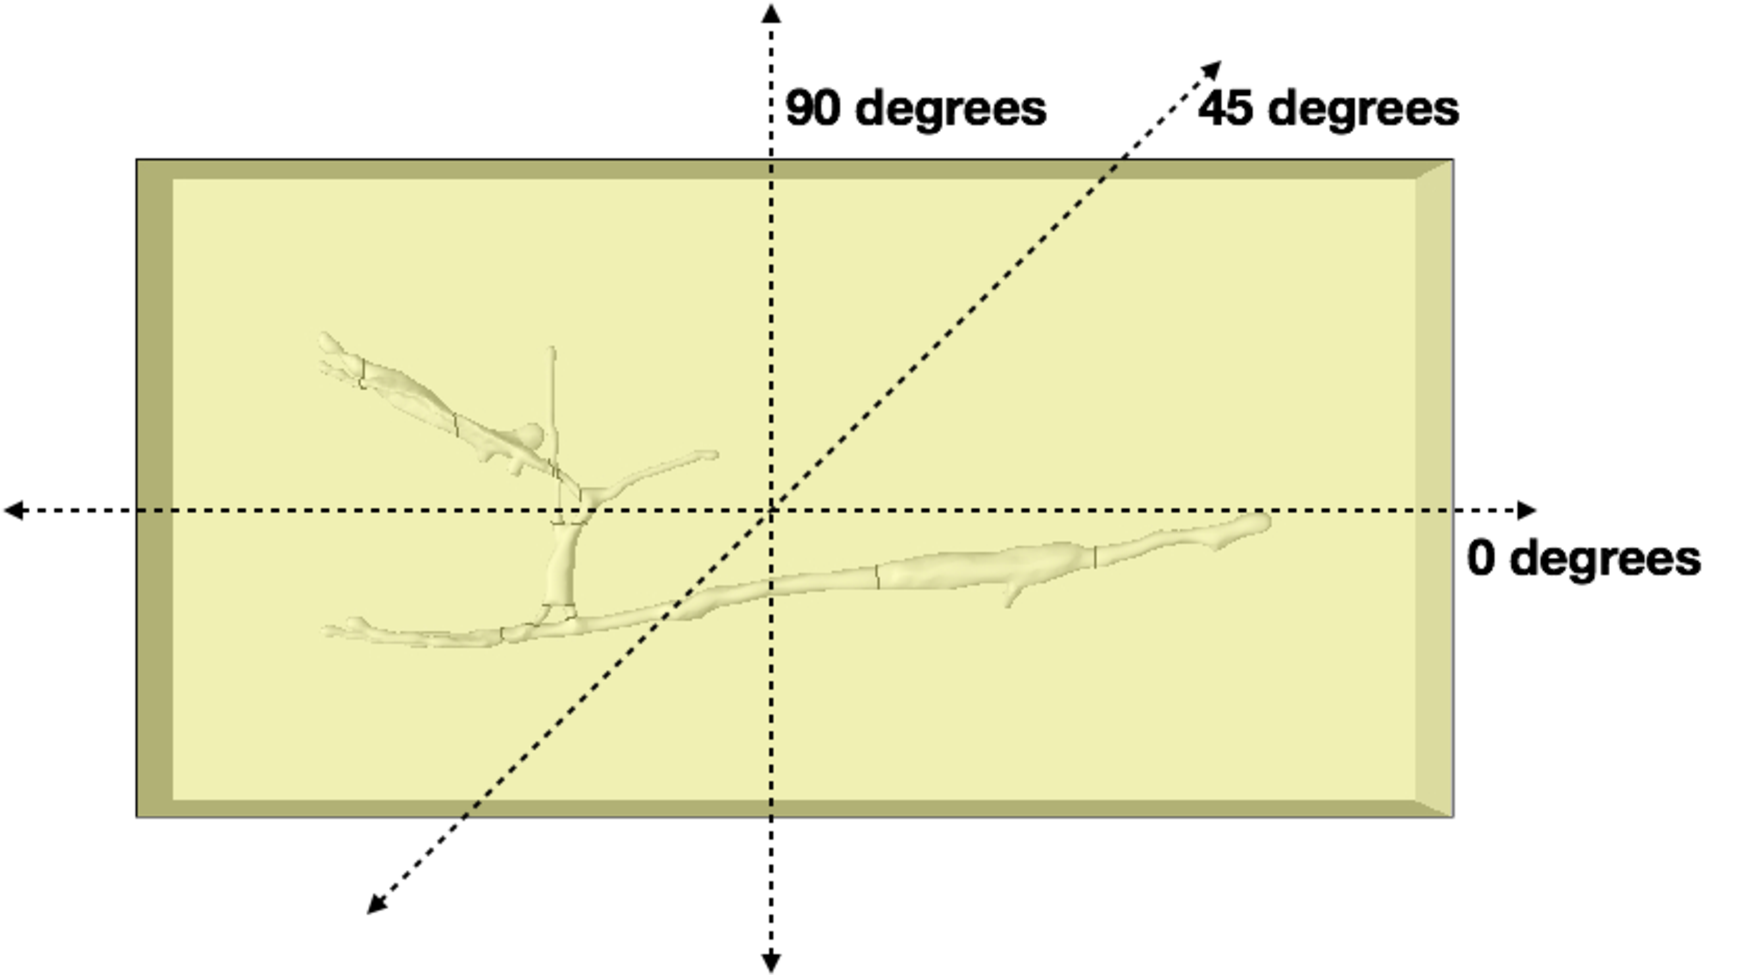
\includegraphics[height=6cm]{figure/AngleLoadingSchematic.pdf} \\
\end{array}
$
\end{center}
\caption{\label{fig:loading_direction} Schematic showing axes of load directions corresponding to $0^{\circ}$, $45^{\circ}$, and $90^{\circ}$ and regions of neuron corresponding to different local axes.}
\end{figure}
%

The strain within the neuron is quantified by a complementary cumulative distribution function (ccdf) defined as 
%
\begin{equation}
\text{ccdf}(X) = \int_{X}^{\infty} p_{\epsilon^*}(X)d\epsilon^* = \text{Pr}[ \epsilon^*\ge X],
\label{eq:ccdf}
\end{equation}
%
where $p_{\epsilon^*}(X)$ is the probability density function of $\epsilon^*$ and $\epsilon^*$ is either the axial, $\epsilon_{\text{ax}}$, or transverse, $\epsilon_{\text{trns}}$, strain with respect to the local axon axis; the four regions corresponding to the different local axes in the neuron are shown schematically in Fig.\ \ref{fig:loading_direction}. Equation \ref{eq:ccdf} is the probability that the neuron (approximately equal to the volume fraction of the neuron) experiences an axial or transverse strain of \textit{greater than or equal to} $X$. In the analysis below, the Green-Lagrange strain was used for measuring deformation.

%=========================================================================================================
\subsection{Varying Axial Stiffness ($t$) in the Cell Body}
\label{sec:cellbody_stiffness}

The ccdfs for different axial stiffnesses of the cell body (different values of $t$) are plotted in Fig.\ \ref{fig:neuron_ccdf_vary_a} for the $0^{\circ}$ loading case for a grip strain of 16$\%$ on the collagen gel. 
%
% Figures generated in SCOREC/Choose-CellStiffness/Compare-CellStiffness folder
\begin{figure}[ht]
\begin{center}
$
\begin{array}{cc}
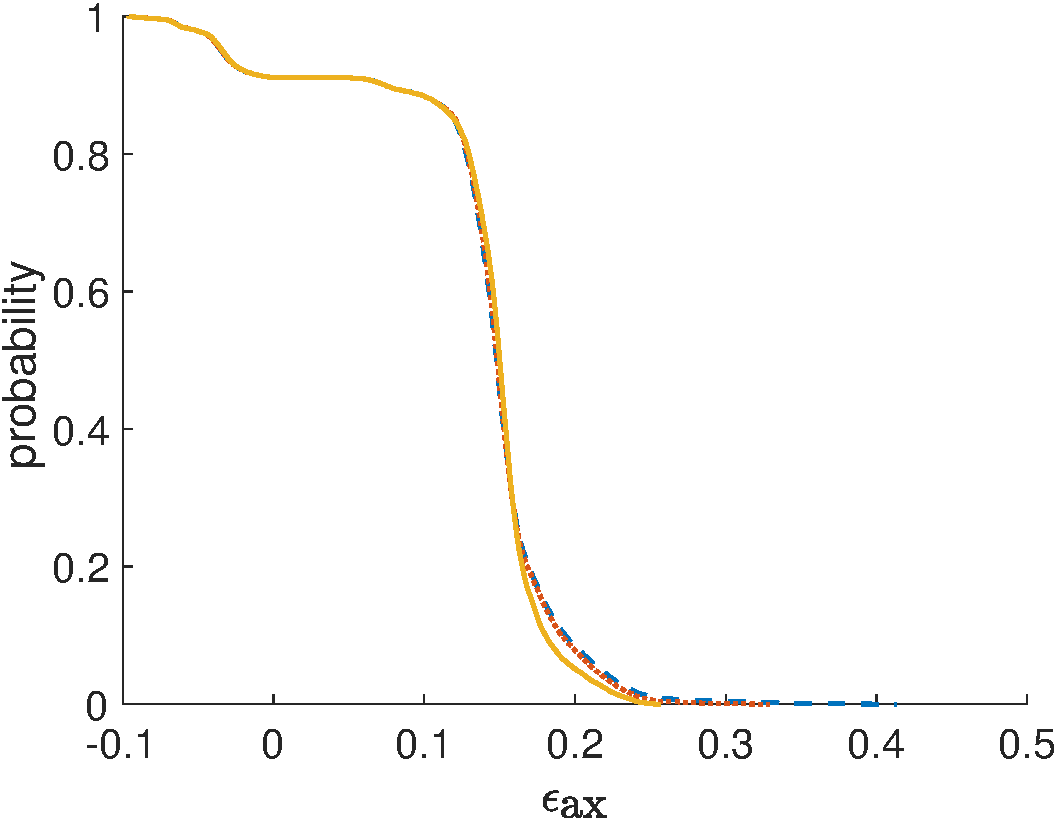
\includegraphics[height=5cm]{figure/neuron_compare_t_ccdf_axial.pdf} &
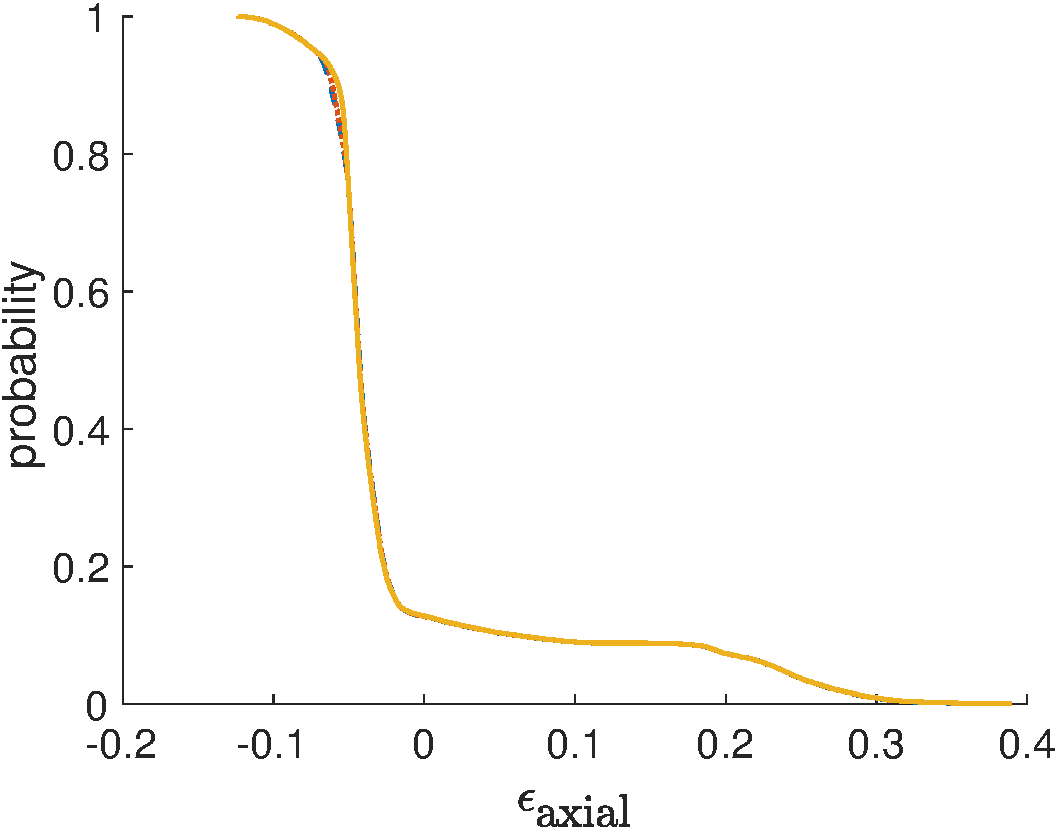
\includegraphics[height=5cm]{figure/neuron_compare_t_ccdf_trns.pdf} \\
(a) & (b)
\end{array}
$
\end{center}
\caption{\label{fig:neuron_ccdf_vary_a} Complimentary cumulative distribution functions for (a) axial and (b) transverse strains in the neuron due to a $0^{\circ}$ load of 16$\%$ grip strain. The distributions are for axial cell-body stiffnesses corresponding to t=28 $\mu$m (blue dashed line), 30 $\mu$m (red dotted line), and 50 $\mu$m (yellow solid line). }
\end{figure}
%
These results suggest that the strain distribution within the neuron is insensitive to the axial stiffness of the cell body. The negative values of strain seen in the distributions are due to lateral contraction that arises from the Poisson effect. 

%=========================================================================================================
\subsection{Strain Distribution within Neuronal Bodies}
\label{subsec:strain_distribution}

The axial and transverse strain distributions in the neuron are examined for the three different loading conditions shown in Fig.\ \ref{fig:loading_direction} for $t=30$ $\mu$m. Color maps of the maximum principal strain in the neuron for a grip strain of 16$\%$ (painful ligament loading) and for $0^{\circ}$, $45^{\circ}$, and $90^{\circ}$ loading are plotted in Fig.\ \ref{fig:neuron_MPS}.
%
% Images from Green-Lagrange-Strain/MaxPrnStrn folder.
\begin{figure}[ht]
\begin{center}
$
\begin{array}{c}
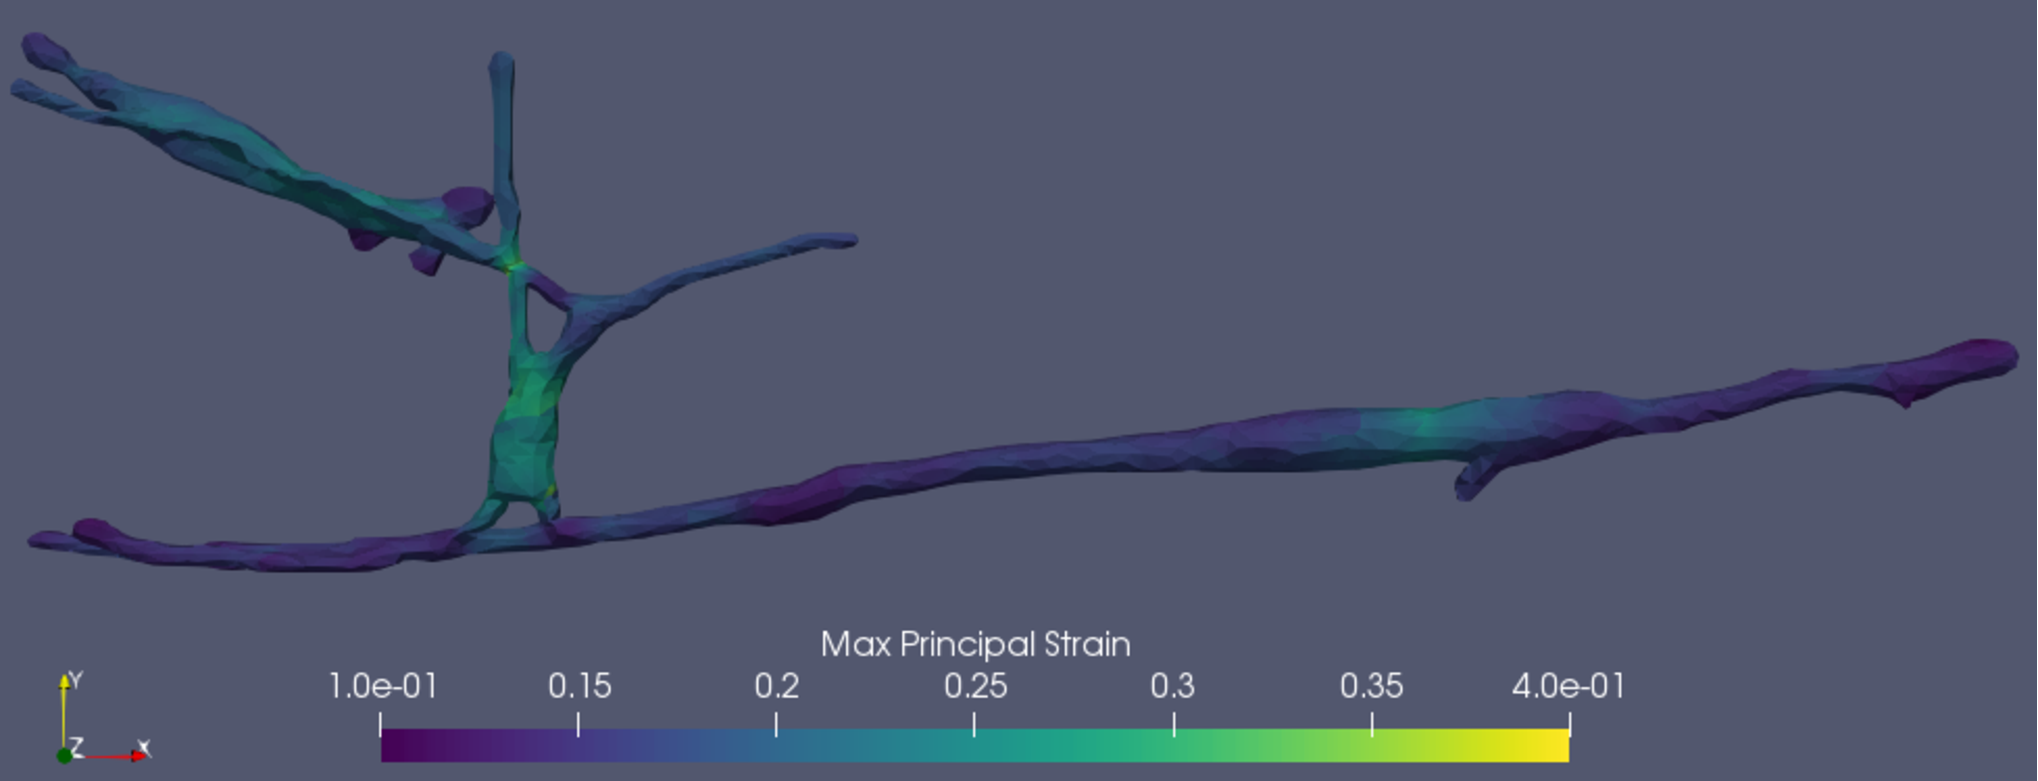
\includegraphics[height=4cm]{figure/rot0_FT50_stp13.pdf} \\
(a) \\
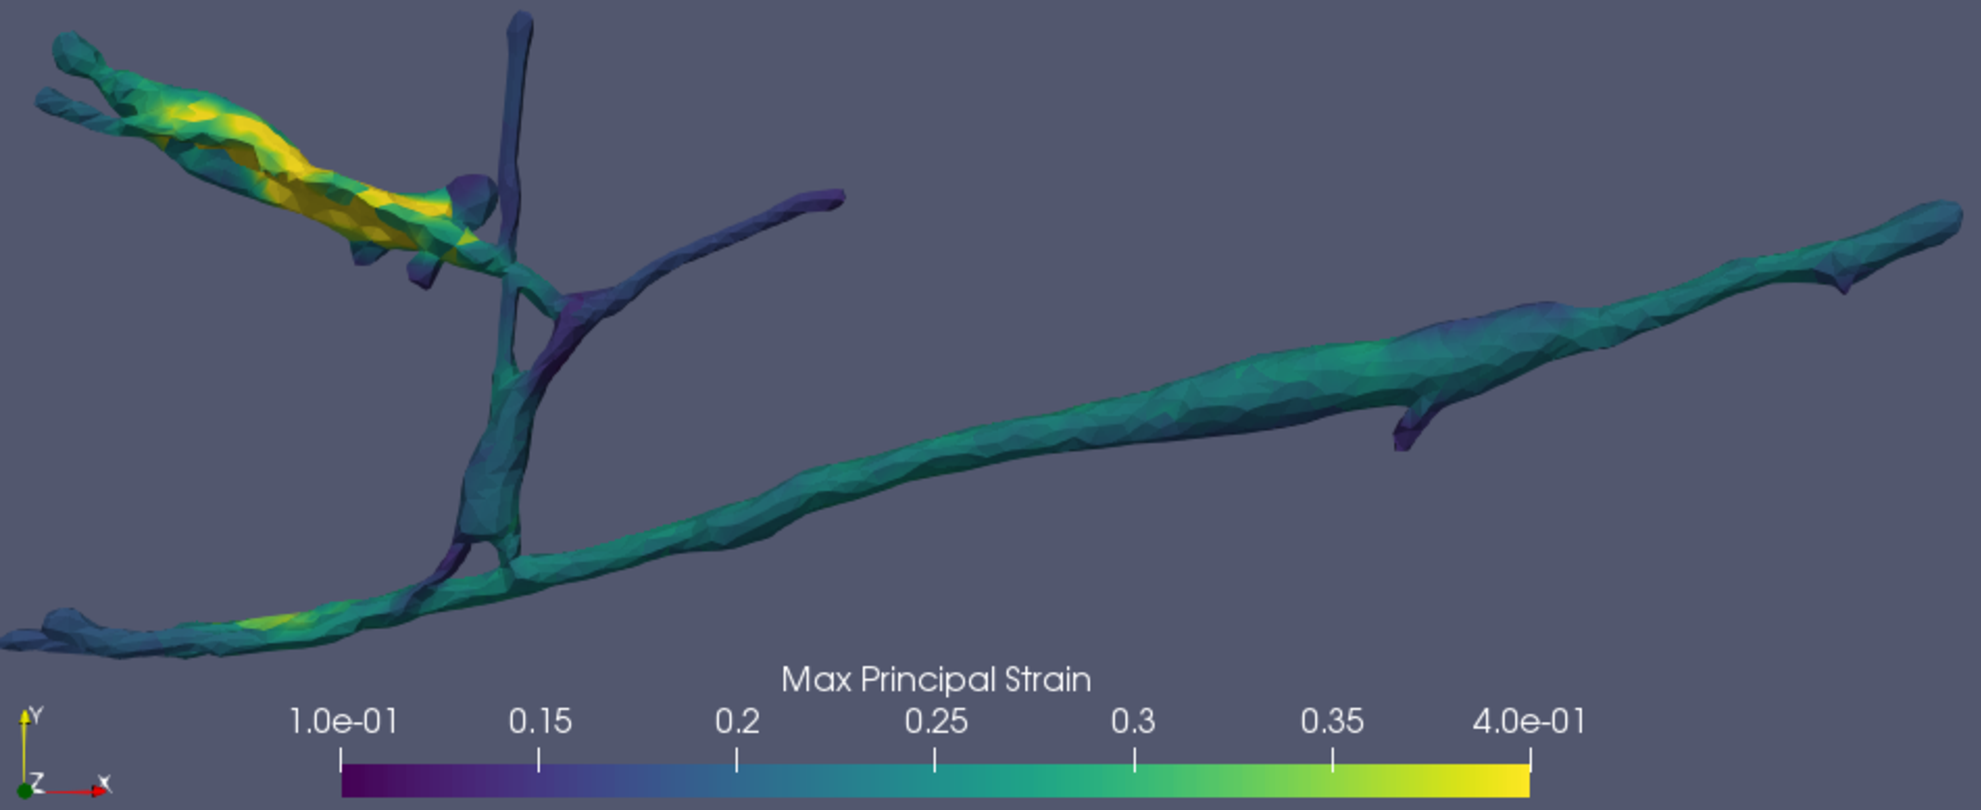
\includegraphics[height=4cm]{figure/rot45_FT50_stp46.pdf} \\
(b) \\
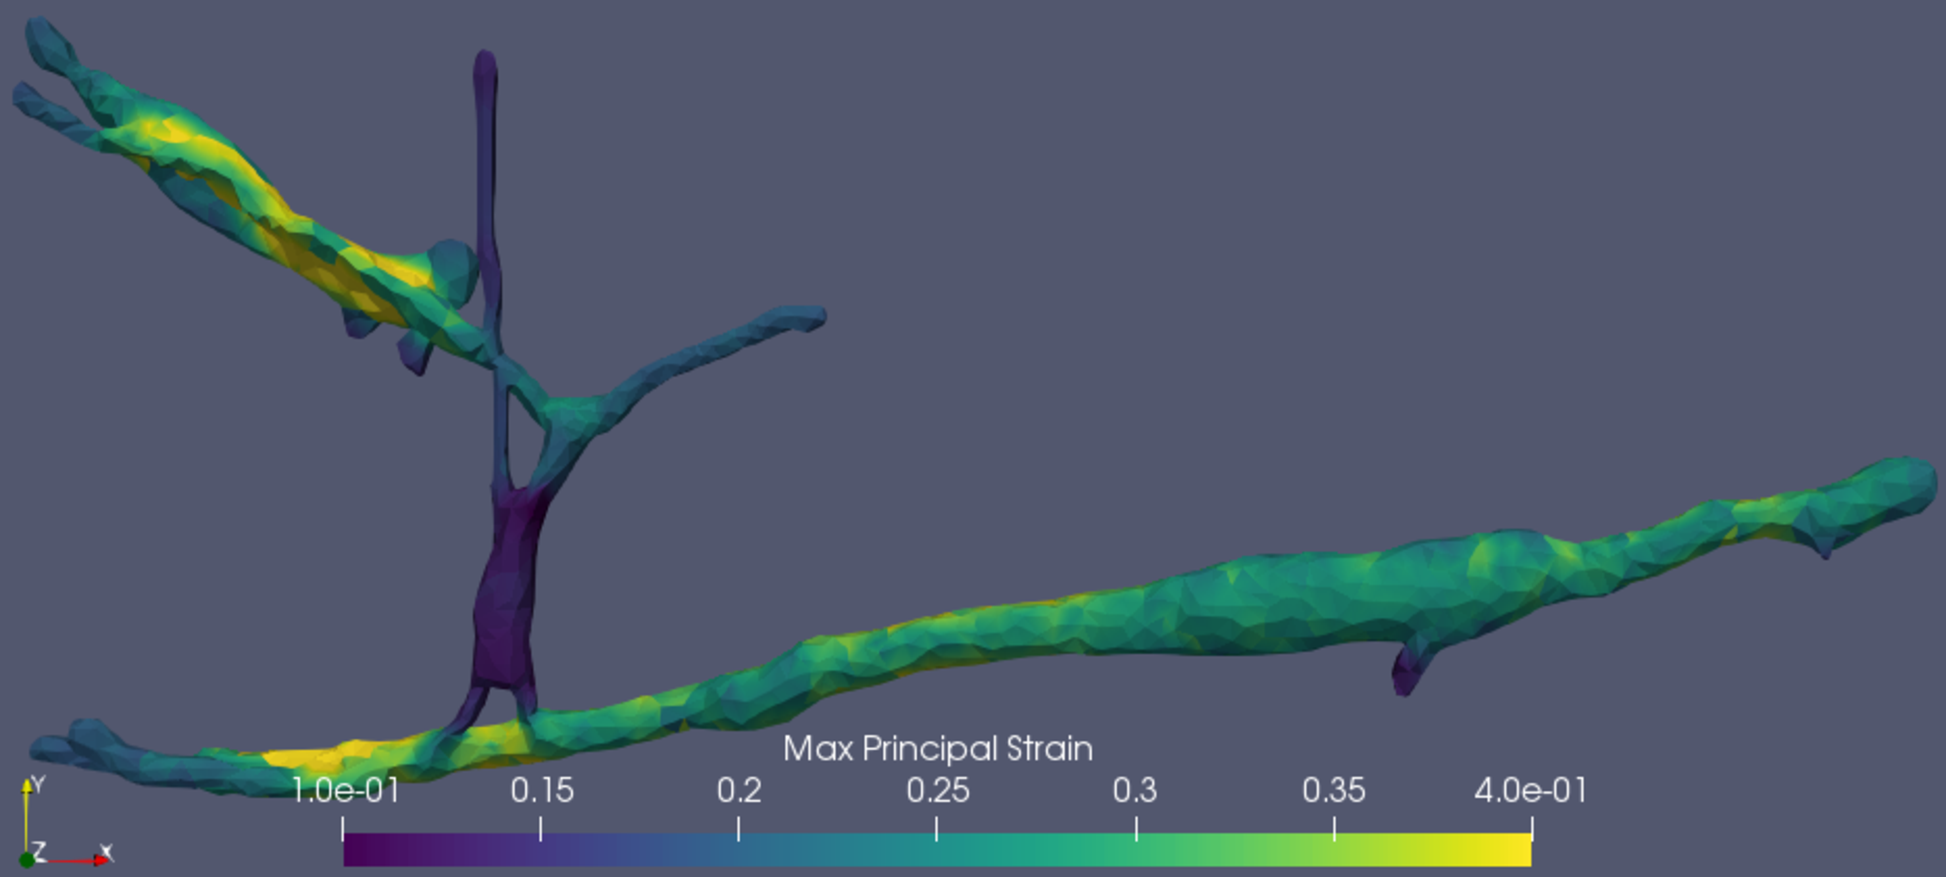
\includegraphics[height=4cm]{figure/rot90_FT50_stp36.pdf} \\
(c)
\end{array}
$
\end{center}
\caption{\label{fig:neuron_MPS} Color maps of MPS in neuron for grip strain of 16$\%$ for loading angles of (a) $0^{\circ}$, (b) $45^{\circ}$, and (c) $90^{\circ}$. The color bar ranges from 10$\%$ to 40$\%$ MPS.}
\end{figure}
%
For all angles of loading, large portions of the neuron experience strains that are greater than the 16$\%$ applied grip strain. This indicates that the applied strains on the collagen gel are amplified in the neuron, which could lead to neuronal damage even when the surrounding tissue is moderately loaded. 

To gain a more quantitative understanding of the strain distribution in the neuron, the ccdfs of the normal strains in the axial and transverse of the axon axis for 10$\%$ (non painful ligament loading) and 16$\%$ (painful ligament loading) grip strains and loading angles of $0^{\circ}$, $45^{\circ}$, and $90^{\circ}$ are plotted in Fig.\ \ref{fig:strain_ccdfs}.
%
% Figure generated in Green-Lagrange-Strain/AxialStrn or TrnsStrn folders
\begin{figure}[ht]
\begin{center}
$
\begin{array}{cc}
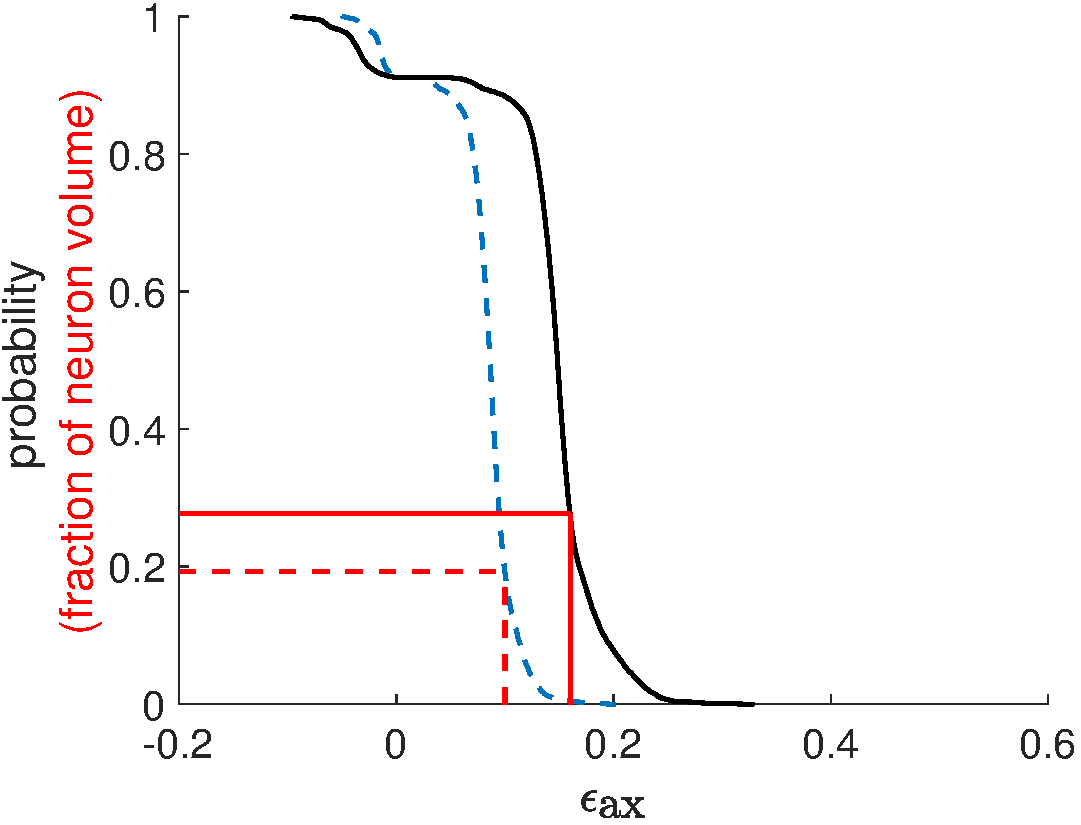
\includegraphics[height=5cm]{figure/angle0_combined_axial.pdf} &
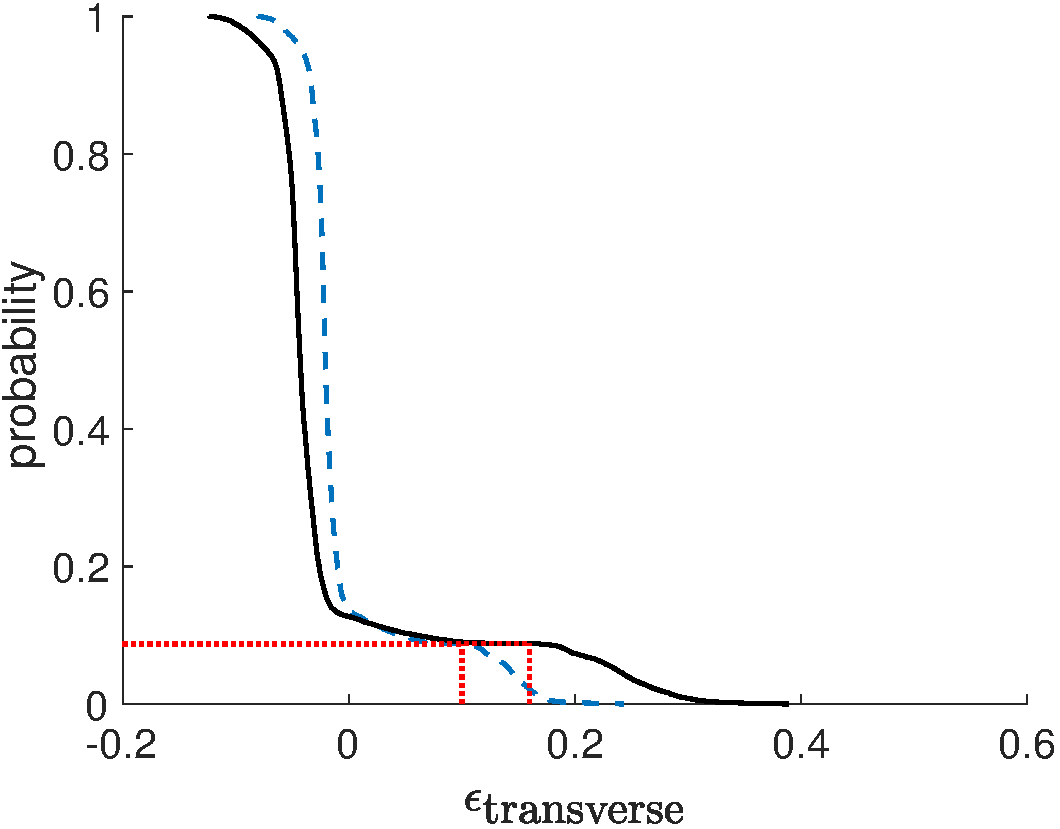
\includegraphics[height=5cm]{figure/angle0_combined_trns.pdf} \\
(a) & (b) \\
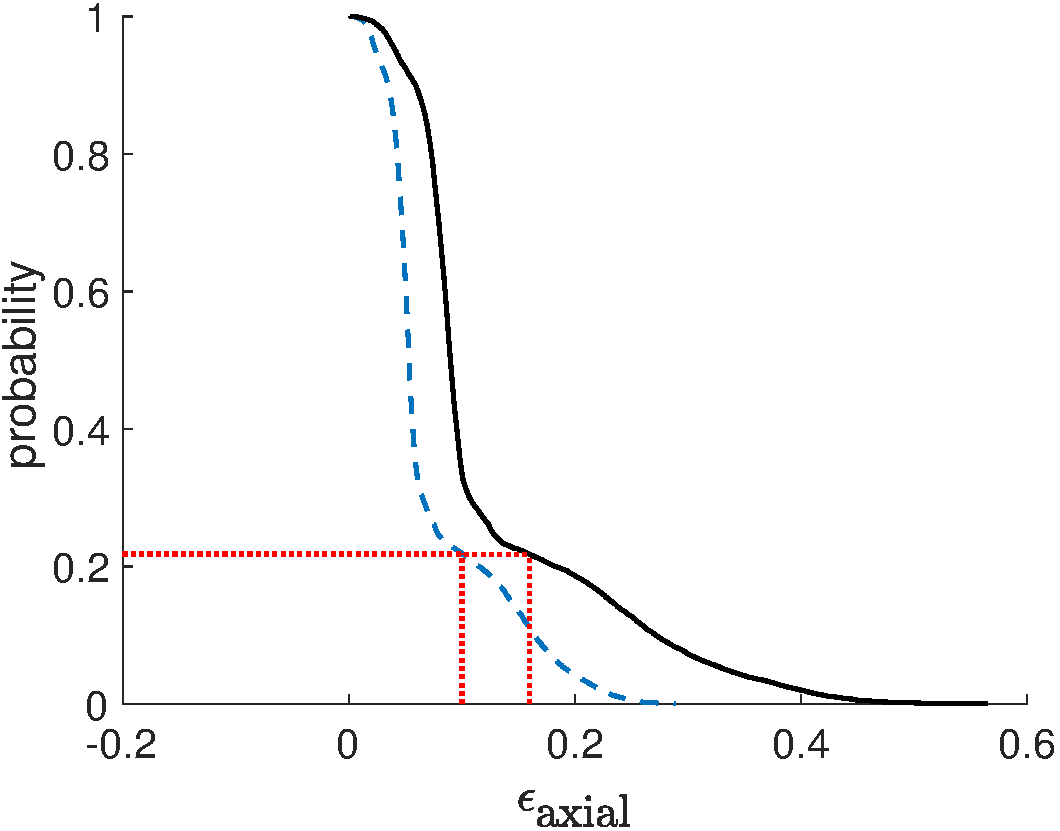
\includegraphics[height=5cm]{figure/angle45_combined_axial.pdf} &
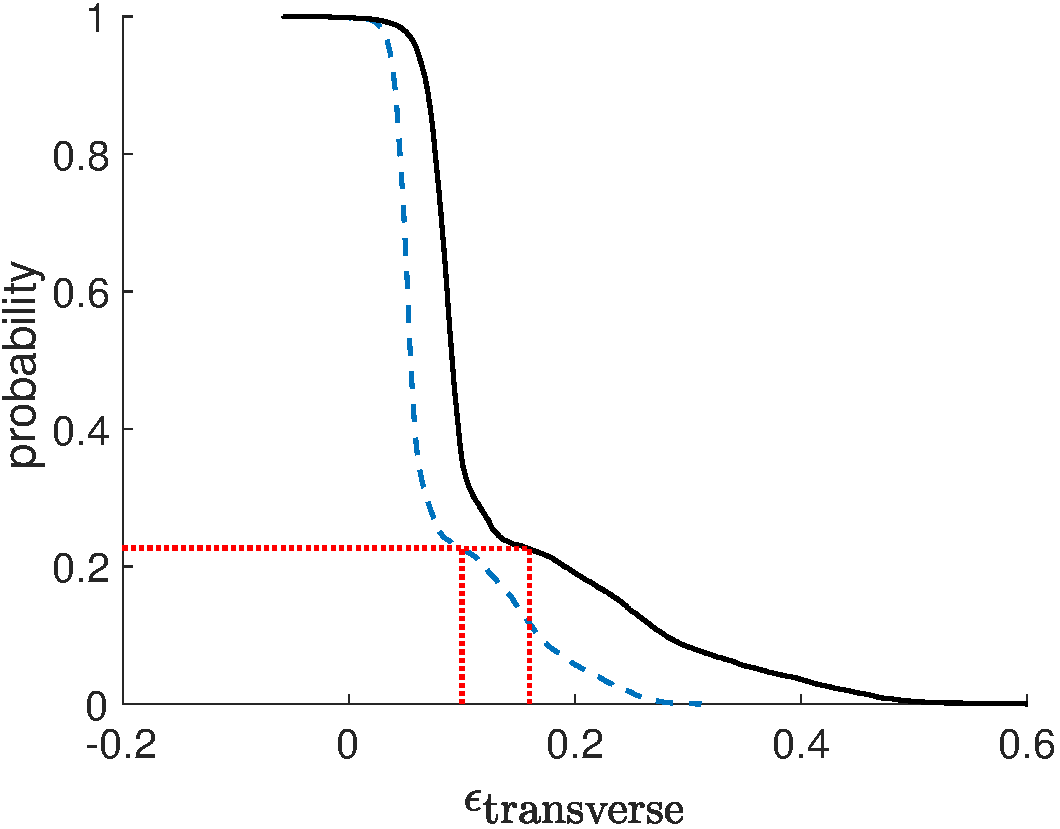
\includegraphics[height=5cm]{figure/angle45_combined_trns.pdf} \\
(c) & (d) \\
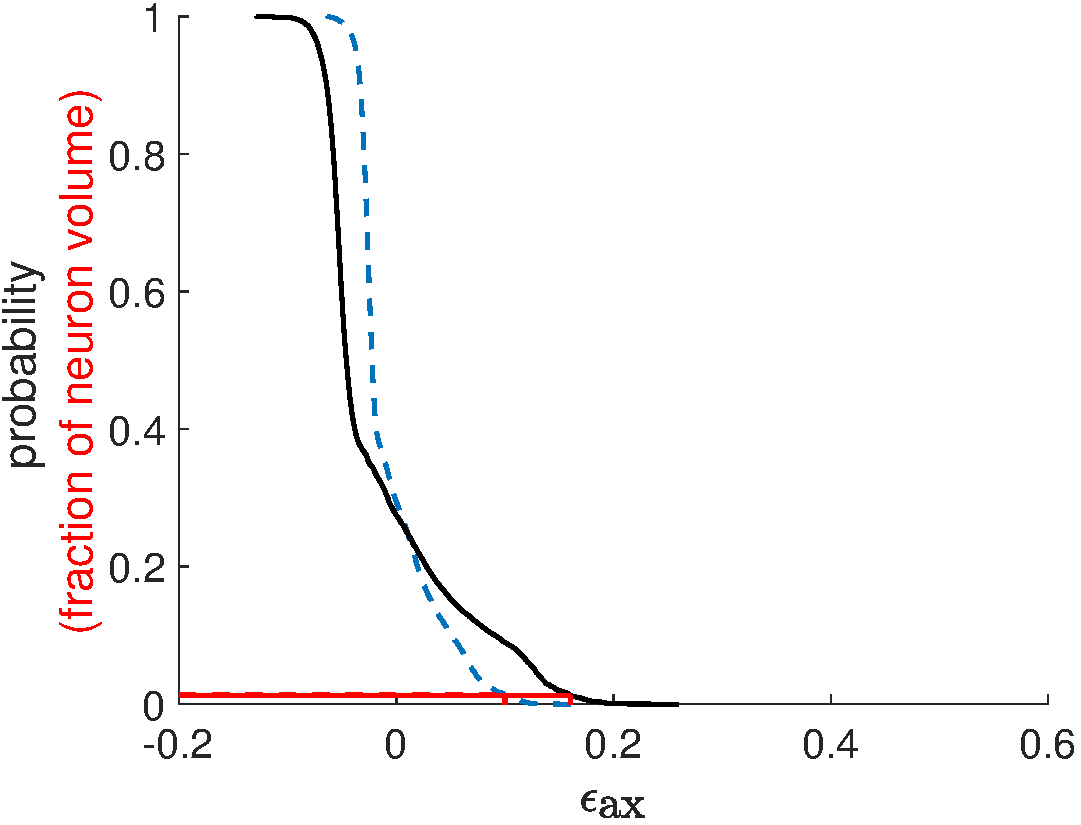
\includegraphics[height=5cm]{figure/angle90_combined_axial.pdf} &
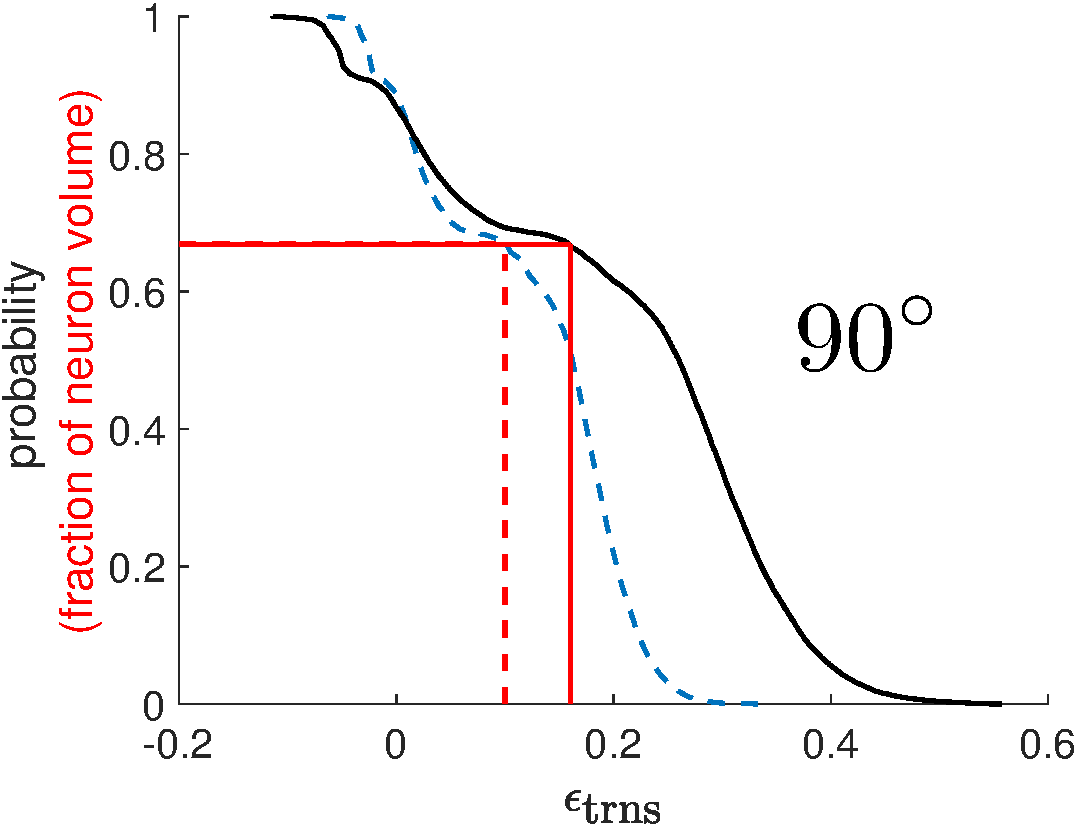
\includegraphics[height=5cm]{figure/angle90_combined_trns.pdf} \\
(e) & (f) 
\end{array}
$
\end{center}
\caption{\label{fig:strain_ccdfs} Complementary cumulative distribution functions for axial (left column) and transverse (right column)  strains in neuron for $0^{\circ}$ (top row), $45^{\circ}$ (middle row), and $90^{\circ}$ (bottom row) loading. Distributions for 10$\%$ (blue dashed line) and 16$\%$ (black solid line) grip strains are plotted for all loading directions. The dashed and solid red lines indicate the approximate fraction of the neuron volume that experience a strain of greater than or equal to 10$\%$ and 16$\%$, respectively. }
\end{figure}
%
As observed in Fig.\ \ref{fig:strain_ccdfs}, the shape of the strain distributions vary significantly for different applied strains and loading directions. The strong dependence of the strain distribution on loading configuration reflects the anisotropic nature of the embedded neuron, where the axial stiffness is more than one order of magnitude greater than the transverse stiffness. Relative to the stiffness of the surrounding collagen gel, the axial stiffness of the neuron is larger while the transverse stiffness of the neuron is smaller. 


%Due to its complex geometry, the embedded neuron is exposed to both transverse and axial components of loading. The spread of the ccdfs reflects the range of tranverse and axial loads that different regions within the neuron experience, both in tension (positive values) and in compression (negative values). Since the ccdfs are measured for strains that are either parallel or perpendicular to the local axial direction of the neuron, 
%
%The range of strains experienced by the neuron in tension and compression are listed in Table \ref{table:ccdf_spread_compare}.
%%
%%%%%%%%%%%%%%%%%%%%%%%%%%%%%%%%%%%%%%%%%%%%%%%%%%%%%%%%%
%\begin{table}[ht]
%\begin{center}
%\begin{tabular}{ c c c c c }
%\hline\hline
%& \multicolumn{2}{c}{axial strain} & \multicolumn{2}{c}{transverse strains} \\ \hline 
%Loading Direction & $\epsilon_{\text{grip}}=0.1$ & $\epsilon_{\text{grip}}=0.16$ & $\epsilon_{\text{grip}}=0.1$ & $\epsilon_{\text{grip}}=0.16$ \\
%\hline 
%\multicolumn{5}{c}{Range in tension} \\ \hline
%0 deg. & 0.20 & 0.33 & 0.24 & 0.39\\ 
%45 deg. & 0.11 & 0.18 & 0.31 & 0.60\\
%90 deg. & 0.16 & 0.26 & 0.34 & 0.56\\ \hline 
%%
%\multicolumn{5}{c}{Range in compression} \\ \hline 
%0 deg. & 0.05 & 0.10 & 0.08 & 0.12\\ 
%45 deg. & 0.03 & 0.06 & 0.04 & 0.06\\
%90 deg. &  0.06 & 0.13 & 0.06 & 0.11\\ \hline \hline
%\end{tabular}
%\end{center}
%\caption{Range of strain values experienced by neuron in tension and compression. The range is defined by $\max(\epsilon_x) - \min(\epsilon_x)$ where $x = $ tension or compression. }
%\label{table:ccdf_spread_compare}
%\end{table}
%%%%%%%%%%%%%%%%%%%%%%%%%%%%%%%%%%%%%%%%%%%%%%%%%%%%%%%%%
%%
%In tension, the largest and smallest range for axial strains is experienced in the 45 and 90 degree loading cases, respectively. On the other hand, the largest and smallest range for transverse strains is experienced in the 90 degree and 45 degree loading cases, respectively. \blue{what does range size physically mean?}
%
%The neuron does not experience compression in the axial direction when loaded at 45 degrees. 

In all cases, the strain magnitude within the neuron is largest for an applied strain of 16$\%$, as expected; the black solid curve lies to the right (left) of the blue dashed curve for positive (negative) values of strain. Interestingly, aside from the axial strain case for $0^{\circ}$ loading, the same fraction of the neuron volume experiences a strain that is greater than or equal to the applied grip strain for each loading direction; the red dashed and solid lines intersect the same value on the ordinate of the ccdf. In the case of axial strain for $0^{\circ}$ loading, the fraction of the neuron volume that amplifies the applied strain increases with grip strain. 

The fraction of the neuron volume that experiences a value of the strain greater than or equal to the far-field applied strain are listed in Table \ref{table:ccdf_volfrac_compare} for all cases plotted in Fig.\ \ref{fig:strain_ccdfs}.
%
%%%%%%%%%%%%%%%%%%%%%%%%%%%%%%%%%%%%%%%%%%%%%%%%%%%%%%%%
\begin{table}[ht]
\begin{center}
\begin{tabular}{ c c c c c }
\hline\hline
& \multicolumn{2}{c}{axial strain} & \multicolumn{2}{c}{transverse strains} \\ \hline 
Loading Direction & $\epsilon_{\text{grip}}=0.1$ & $\epsilon_{\text{grip}}=0.16$ & $\epsilon_{\text{grip}}=0.1$ & $\epsilon_{\text{grip}}=0.16$ \\
\hline 
$0^{\circ}$ & 19$\%$ & 28$\%$ & 9$\%$ & 9$\%$\\ 
$45^{\circ}$ & 0$\%$ & 0$\%$ & 23$\%$ & 23$\%$\\
$90^{\circ}$ & 13$\%$ & 13$\%$ & 67$\%$ & 67$\%$\\ \hline \hline
\end{tabular}
\end{center}
\caption{Fraction of the neuron volume that experiences a strain that is greater than or equal to the applied strain on surrounding collagen gel for different loading directions.}
\label{table:ccdf_volfrac_compare}
\end{table}
%%%%%%%%%%%%%%%%%%%%%%%%%%%%%%%%%%%%%%%%%%%%%%%%%%%%%%%%
%
As seen in Table \ref{table:ccdf_volfrac_compare}, the applied strain on the collagen gel is amplified in the neuron predominantly along the axial direction for $0^{\circ}$ loading and in the transverse direction for $45^{\circ}$ and $90^{\circ}$ loading. For $45^{\circ}$ loading, less than 0.1$\%$ of the neuron volume experiences an axial strain that is greater than or equal to the applied strain.

The values listed in Table \ref{table:ccdf_volfrac_compare} are consistent with how the embedded neuron is oriented relative to the different loading directions. When loading at $0^{\circ}$ a majority of the neuron volume (regions 1, 2, and 4 in Fig.\ \ref{fig:loading_direction}) are loaded predominantly in the axial direction giving rise to the largest fraction of neuron volume that amplifies the applied strain in the axial direction. On the other hand, when loading at $90^{\circ}$ a majority of the neuron volume (regions 1, 3, and 4 in Fig.\ \ref{fig:loading_direction}) are loaded predominantly in the transverse direction giving rise to the largest fraction of neuron volume that amplifies the applied strain in the transverse direction. The amplification of the applied strain in the transverse direction is significantly greater because the neuron is much softer in the transverse direction relative to the axial direction.  The neuron also experiences a significant strain amplification in the transverse direction when loaded at $45^{\circ}$ because the axial direction of region 1 lies perpendicular to the $45^{\circ}$ loading direction.

Physiologically more important are the tails of the strain distributions which represent the largest strains experienced by the neuron. The strain values corresponding to the largest 10$\%$ (by neuron volume) of deformation in the neuron are listed in Table \ref{table:ccdf_tail_strains}. 
%
%%%%%%%%%%%%%%%%%%%%%%%%%%%%%%%%%%%%%%%%%%%%%%%%%%%%%%%%
\begin{table}[ht]
\begin{center}
\begin{tabular}{ c c c c c }
\hline\hline
& \multicolumn{2}{c}{Largest 10$\%$ of axial strain} & \multicolumn{2}{c}{Largest 10$\%$ of transverse strain} \\ \hline 
Loading Direction & $\epsilon_{\text{grip}}=0.1$ & $\epsilon_{\text{grip}}=0.16$ & $\epsilon_{\text{grip}}=0.1$ & $\epsilon_{\text{grip}}=0.16$ \\
\hline 
$0^{\circ}$ & $0.11^*$ & $0.19^*$ & 0.04 & 0.06\\ 
$45^{\circ}$ & $0.06$ & $0.10$ & $0.17^*$ & $0.28^*$\\
$90^{\circ}$ & 0.05 & 0.09 & $0.22^*$ & $0.37^*$\\ \hline \hline
\end{tabular}
\end{center}
\caption{Strain values corresponding to the largest 10$\%$ of deformation in the neuron. Asterisks indicate strain values that are greater than the applied strain, i.e., applied strain is amplified within neuron.}
\label{table:ccdf_tail_strains}
\end{table}
%%%%%%%%%%%%%%%%%%%%%%%%%%%%%%%%%%%%%%%%%%%%%%%%%%%%%%%%
%
Consistent with above, the applied strain is amplified along the axial direction for $0^{\circ}$ loading and the transverse direction for $45^{\circ}$ and $90^{\circ}$ loading. Of these cases, the largest and smallest amplifications arise for $90^{\circ}$ and $0^{\circ}$ loading, respectively.

When loaded at $90^{\circ}$, 10$\%$ of the neuron volume experiences a strain amplification of at least 2$\times$ in the transverse direction. When loaded at $45^{\circ}$, the same fraction of the neuron volume experiences an amplification of at least 1.7$\times$. When loaded at $0^{\circ}$, 10$\%$ of the neuron volume experiences a strain amplification of at least 1.1$\times$ in the axial direction. The smaller amplification in the axial direction is due to the larger stiffness of the neuron in the axial direction relative to the transverse direction. 

%%%%%%%%%%%%%%%%%%%%%%%%%%%%%%%%%%%%%%%%%%%%%%%%%%%%%%%%%%%%%%%%%%%%%%
\section{Summary}
\label{sec:summary}

We have presented a general modeling strategy in which (1) a realistic representation of a complex cell geometry is generated from confocal microscopy images of DRG neurons embedded in a collagen gel; (2) the geometric model is converted into a finite-element mesh; (3) a multi-scale model is implemented in the mesh corresponding to the extracellular matrix (collagen gel); and (4) an analysis of the strain distributions within the neuron due to mechanical loading on the extracellular matrix.

The large computational demands that arise from the unstructured mesh of a complex cell geometry coupled by with a multi-scale model is accommodated through the AMSI library, which is used to manage the parallel execution spaces of the macroscopic and microscopic scale simulation codes and to plan and enact the necessary parallel communication operations in order to couple the two separate codes together into a multi-scale simulation.

The simulation results for the embedded neuron provides local strain information that is not accessible by current experimental techniques, thereby providing important insights about the mechanism of neuronal injury under mechanical loading. We find that the strain distribution in the neuron depends strongly on the configuration of the embedded neuron relative to the loading direction, which reflects the anisotropic mechanical properties of the neuron. More importantly, we observe that the applied strain on the surrounding environment is amplified within the neuron for all loading configurations considered. In the most severe cases, the applied strain is amplified by at least 2$\times$ in 10$\%$ of the neuron volume. 

The work presented in this paper provides an extension to the capability of past modeling strategies by enabling the realistic representation of complex cell geometry into a multi-scale framework. Although several physiologically important mechanisms for the embedded neuron system has been left out, e.g., \red{Sijia, Beth, Victor B.: can you help with this?}, the results from the simplified system nonetheless provide meaningful results that can be built upon in future work.

\red{Sijia, Beth, Victor B.: How representative is this one neuron configuration that we study? Can we extrapolate these results to other studies?} 


%%%%%%%%%%%%%%%%%%%%%%%%%%%%%%%%%%%%%%%%%%%%%%%%%%%%%%%%%%%%%%%%%%%%%%
%\begin{acknowledgment}
%\begin{enumerate}
%\item{NIH Grants}
%\item{Computing resources were provided by the Center for Computational Innovations at Rensselaer Polytechnic Institute \red{Will check specific wording on CCI website.}}
%\end{enumerate}
%\end{acknowledgment}

%%%%%%%%%%%%%%%%%%%%%%%%%%%%%%%%%%%%%%%%%%%%%%%%%%%%%%%%%%%%%%%%%%%%%%
% The bibliography is stored in an external database file
% in the BibTeX format (file_name.bib).  The bibliography is
% created by the following command and it will appear in this
% position in the document. You may, of course, create your
% own bibliography by using thebibliography environment as in
%
% \begin{thebibliography}{12}
% ...
% \bibitem{itemreference} D. E. Knudsen.
% {\em 1966 World Bnus Almanac.}
% {Permafrost Press, Novosibirsk.}
% ...
% \end{thebibliography}
\newpage
% Here's where you specify the bibliography style file.
% The full file name for the bibliography style file 
% used for an ASME paper is asmems4.bst.
%%\bibliographystyle{asmems4}
\bibliographystyle{tfcse}

% Here's where you specify the bibliography database file.
% The full file name of the bibliography database for this
% article is asme2e.bib. The name for your database is up
% to you.
\bibliography{references}


%%%%%%%%%%%%%%%%%%%%%%%%%%%%%%%%%%%%%%%%%%%%%%%%%%%%%%%%%%%%%%%%%%%%%%
\appendix
\section*{Appendix A: Derivation of $P_2$ from $\alpha$ and $\delta$ of the QPLI method}
\label{app:P2_derivation}

Consider a distribution of orientation $\theta$ for pixel $i$ as 
%
\begin{equation}
p_i(\theta) = q_i + r_i\cos^2(\theta - \alpha_i) \ \ \text{for} \ \ \theta \in (0,\pi),
\label{eq:distribution}
\end{equation}
%
where $\alpha_i$ is the alignment measured at pixel $i$ by the QPLI method and $q_i$ and $r_i$ are constants for the $i^{th}$ pixel. Applying the normalization 
%
\begin{equation}
\int_0^{\pi}p_i(\theta)d\theta = 1,
\end{equation}
%
a relationship between $q_i$ and $r_i$ is obtained:
%
\begin{equation}
\pi q_i + \frac{\pi}{2}r_i = 1.
\label{eq:q_relationship}
\end{equation}
%
Using the relationship in Eq.\ \eqref{eq:q_relationship}, Eq.\ \eqref{eq:distribution} can be rewritten as
%
\begin{equation}
p_i(\theta) = q_i + \frac{2}{\pi}(1-\pi q_i)\cos^2(\theta-\alpha_i)
\label{eq:distribution_q}
\end{equation}
%

The orientation tensor for each pixel can be written in terms of $p_i(\theta)$ as
%
\begin{eqnarray}
\pmb{A}^i = 
\begin{bmatrix}
\int_0^{\pi} p_i(\theta) \cos^2(\theta)d\theta & \int_0^{\pi} p_i(\theta) \sin(\theta) \cos(\theta)d\theta \\
\int_0^{\pi} p_i(\theta) \sin(\theta) \cos(\theta)d\theta & \int_0^{\pi} p_i(\theta) \sin^2(\theta)d\theta
\end{bmatrix} = 
%
\frac{1-\pi q_i}{4} 
\begin{bmatrix}
\cos(2 \alpha_i) & \sin(2 \alpha_i) \\
\sin(2\alpha_i) & - \cos(2\alpha_i)
\end{bmatrix},
\label{eq:Ai}
\end{eqnarray}
%
where the eigenvalues of $\pmb{A}^i$ are
\begin{equation}
\lambda_1 = \frac{1+\pi q_i}{4} \ \ \text{and} \ \ \lambda_2 = \frac{3-\pi q_i}{4}. 
\end{equation}
%
The retardation at each pixel, $\delta_i$, can be calculated from the eigenvalues by
%
\begin{equation}
\delta_i = |\lambda_2 - \lambda_1| = \frac{1-\pi q_i}{2}.
\label{eq:delta_i}
\end{equation}
%
From Eq.\ \eqref{eq:delta_i}, the constant $q_i$ can be written in terms of the retardation as
%
\begin{equation}
q_i = \frac{1}{\pi}(1-2\delta_i),
\end{equation}
%
and the distribution at pixel $i$ from Eq.\ \eqref{eq:distribution_q} can be rewritten as
%
\begin{equation}
p_i(\theta) = \frac{1-2\delta_i}{\pi} + \frac{4 \delta_i}{\pi}\cos^2(\theta-\alpha_i).
\label{eq:distribution_delta}
\end{equation}
%

The distribution of orientation $\theta$ for the entire image is simply the average over the distribution of each pixel
%
\begin{equation}
p(\theta) = \frac{1}{N} \sum_{i=1}^N p_i(\theta) = \frac{1}{N} \sum_{i=1}^N \left[ \frac{1-2\delta_i}{\pi} + \frac{4 \delta_i}{\pi}\cos^2(\theta-\alpha_i) \right],
\end{equation}
%
which is the equation presented in Eq.\ \eqref{eq:P2_experiment}.


\end{document}
